\documentclass[a4paper, openany]{memoir}

\usepackage[utf8]{inputenc}
\usepackage[T1]{fontenc} 
\usepackage[english]{babel}

\usepackage{fancyhdr}
\usepackage{float}

\usepackage{amsmath}
\usepackage{amsthm}
\usepackage{amssymb}
\usepackage{enumitem}
\usepackage{multicol}
\usepackage[bookmarksopen=true,bookmarksopenlevel=2]{hyperref}
\usepackage{tikz}
\usepackage{indentfirst}

\pagestyle{fancy}
\fancyhf{}
\fancyhead[LE]{\leftmark}
\fancyhead[RO]{\rightmark}
\fancyhead[RE, LO]{Data Fundamentals}
\fancyfoot[LE, RO]{\thepage}
\fancyfoot[RE, LO]{Pete Gautam}

\renewcommand{\headrulewidth}{1.5pt}

\chapterstyle{thatcher}
\setcounter{chapter}{3}
\begin{document}

\chapter{Optimisation}
\section{Introduction to Optimisation}
Optimisation is the process of finding the best solution to a question. We would like to create algorithm(s) that given the optimal solution given a problem. These algorithms should be efficient- they should try to study as few possible solutions as they can. We can thinking of optimisation algorithms as searching the solution space and trying to find the best possible solution.

An optimisation algorithm can be applied to any optimisation problem. There are no specific cases depending on the problem. Instead, we give to the algorithm the problem in a way that the right value can be optimised.

\subsection{Parameters and Objective Function}
An optimisation problem has 2 aspects:
\begin{itemize}
    \item a set of parameters: the values we can change to improve the final value. This can be one single value, or an array of values. It is denoted by $\theta$. These parameters exist in some parameter space $\Theta$. This might be a vector space like $\mathbb{R}^n$. If so, we call the parameters $\theta$ a vector, i.e. the parameter vector $\theta$.
    \item the objective function: the function that takes all the parameters and maps it to a single value. This is the value we are trying to optimise (minimise to maximise). The function is denoted by $L$ (and called the loss/objective function), and we want to find the minimum/maximum $L(\theta)$.
\end{itemize}

Therefore, the optimisation process finds the value
\[\theta^* = \operatornamewithlimits{arg min}_{\theta \in \Theta} L(\theta),\]
where:
\begin{itemize}
    \item $\theta^*$ is the optimal solution- the value we are trying to find;
    \item $\Theta$ is the parameter space; and
    \item $\theta$ is a configuration of the parameters, an element in $\Theta$.
\end{itemize}
Most optimisation problems also have an extra aspect- a constraint. This is a limitation to the possible configuration of the parameters. That is, we limit the parameter space into a subspace, which is the feasible set/region of solutions (e.g. the speed of a car cannot be 500km per hour).

We will only consider optimisation processes that minimise a value. We can always make the loss function return the negative value so that the final result will be a maximum.

For example, an optimisation problem can be that we are given a function $f$ which takes in some parameter vector $\theta$ along with a fixed input vector $\mathbf{x}$, and we want to find a particular set of parameters $\theta^*$ such that $f(\mathbf{x}, \theta^*)$ is as close to some value $y$ as possible. In that case, the loss function would try to minimise the distance between $f(\mathbf{x}, \theta)$ and $y$, i.e.
\[L(\theta) = \lVert f(\mathbf{x}, \theta) - y \rVert.\]
It is possible that evaluation the loss function $L$ is expensive, e.g.
\begin{itemize}
    \item it might take a long time to compute the value;
    \item it might require a real world experiment;
    \item it might be dangerous; or
    \item it might require data that cannot be accessed for free.
\end{itemize}
So, a good optimisation algorithm would try to mimise the number of times we call the loss function. To do this, there has to be some (mathematical) structure within the optimisation process.

\section{Discrete and continuous problems}
If the parameters are from a continuous space (e.g. $\mathbb{R}^n$), then problem is continuous optimisation. If the parameters are from a discrete space, then the problem is discrete optimisation. It is easier to optimise in a continuous space since we can make assumptions about the data (using continuity and smoothness).

For example, consider the problem of optimising the angle at which we should throw a stone so that it travels the farthest, considering both gravity and air resistance.
\begin{figure}[H]
    \centering
    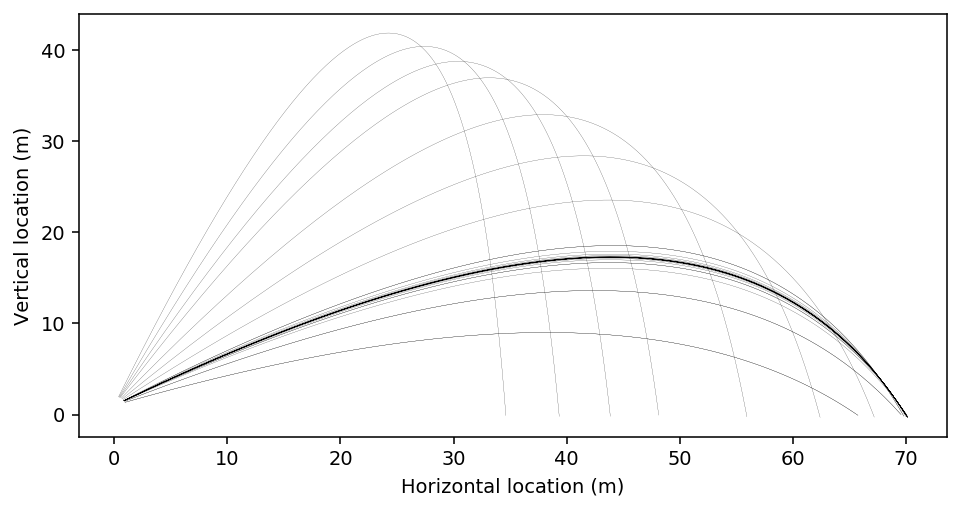
\includegraphics[scale=0.6]{src/4.1 ball optimisation.png}
    \caption{Optimisation the angle of a ball throw.}
\end{figure}
\noindent The optimisation algorithm consider multiple angles (the lighter lines) the ball could be thrown. It concluded that the ball should be thrown at about $30^{\circ}$ to throw it the farthest, denoted by the blue line.

We will focus on continuous optimisation in $\mathbb{R}^n$. So, the parameter
\[\theta = \begin{bmatrix}
    \theta_1 & \theta_2 & \dots & \theta_n
\end{bmatrix},\]
and the optimisation problem satisfies
\[\theta^* = \operatornamewithlimits{arg min}_{\theta \in \mathbb{R}^n} L(\theta),\]
subject to constraints.

Normally, the loss function is smooth and continuous (this is different to $\mathbb{R}^n$ being continuous). There are many classes of optimisation algorithms, such as:
\begin{itemize}
    \item iterative- they generate more optimised solutions with more iterations; and
    \item direct- they can find the minimum in one step.
\end{itemize}

Now, we consider an optimisation algorithm- finding the median of a dataset in $\mathbb{R}^2$. The median can be computed by sorting the dataset and choosing the minimum elment. Another way of thinking about the median is that it minimises the sum of distances to all vectors of the dataset. So, this can be viewed as an optimisation algorithm. Here, the parameter set $\Theta = \mathbb{R}^2$, and we want to find the value $\theta \in \Theta$ such that the value
\[L(\theta) = \sum_i \lVert \theta - \mathbf{x}_i \rVert_2\]
is minimised, where $\mathbf{x}_i$ are the set of 2D points in the dataset (the collection of target points). The following image illustrates this.
\begin{figure}[H]
    \centering
    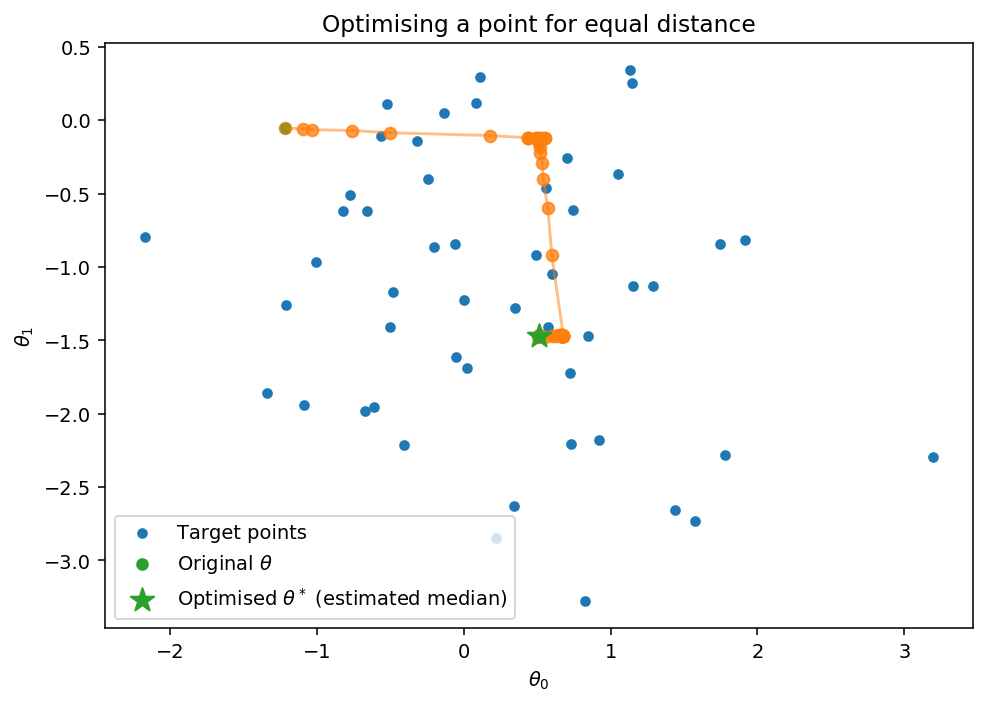
\includegraphics[scale=0.6]{src/4.2 optimising a point to equal distance.png}
    \caption{Finding the minimum of a 2D dataset using optimisation.}
\end{figure}
\noindent Here, the blue points are the values in the dataset. The green point is our inital guess, and we iteratively try to optimise the value- the value we find in each iteration is given in orange. We can use the same idea in higher dimensions.

Now, consider another problem- given a set of points in $\mathbb{R}^n$, we want to find out a layout of points such that the points are evenly spaced. In that case, the parameter space $\Theta = \mathbb{R}^n$, and the loss function is
\[L(\theta) = \sum_i \sum_j (\alpha - \lVert \mathbf{x}_i - \mathbf{x}_j \rVert_2)^2,\]
where $\alpha$ is the space we want most of the points to differ by- we unravel the $\theta$ into vectors $\mathbf{x}_i$ and $\mathbf{x}_j$. This will try to find a configuration of points that are all $\alpha$ units apart, as shown below.
\begin{figure}[H]
    \centering
    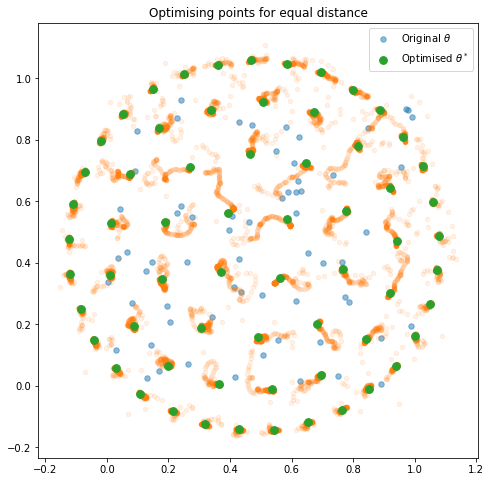
\includegraphics[scale=0.5]{src/4.3 optimising points for equal distance.png}
    \caption{Optimising points in $\mathbb{R}^2$ for equal distance.}
\end{figure}

\section{Constrained optimisation}
The constrained optimisation equation is
\[\theta^* = \operatornamewithlimits{arg min}_{\theta \in \Theta} L(\theta), \text{ subject to } c(\theta) = 0,\]
where $c$ is the constraint function. Alternatively, we can have
\[\theta^* = \operatornamewithlimits{arg min}_{\theta \in \Theta} L(\theta), \text{ subject to } c(\theta) \leq 0.\]
An equality constraint can be constraining a value to some surface, while an inequality constraint is like constraining the value to a volume.

A box constraint is just the requirement that $\theta$ lies in some $\mathbb{R}^n$, e.g. $\theta_i$ is between 0 and 1 (the unit cube), or $\theta_i$ is positive (in the positive orthant). A convex constraint is another constraint with just inequalities on a convex sum of parameters $\theta$- it can be thought of as the intersection of (hyper)planes. Box constraint is a specific type of a convex constraint.

Unconstrained optimisation has no constraints. Typically, the values returned by unconstrained optimisation is not helpful/feasible in real life. There are 2 way of implementing a constrained optimisation problem- purely constrained one or penalty approach. 

In a pure constrained approach, we use an optimisation algorithm that implements hard constraints inherently. This might be straightforward in some cases, but is difficult in most. Typically, constraints will be specified as either a convex region or a simple (hyper)rectangular region of the space (a box constraint). Using constrained optimisation, we can guarantee that the solution is feasible (i.e. it obeys the constraints). It might also mean that we perform fewer computations (since there are fewer possible outcomes). However, it may be less efficient than an unconstrained optimisation; there are fewer algorithms that can be used to optimise; and it can be hard to specify the constraint to the optimiser.

In a soft constraint approach, we can add a penalty term to the loss function to discourage solutions that do not match the constraints. It is more appropriate if there is no set boundary of constraints (e.g. it doesn't matter if the values are just one a bit out of the constraint). We modify the loss function to
\[L(\theta') = L(\theta) + \lambda(\theta),\]
where $\lambda$ is the penalty function. As the value gets further from the constraint, the penalty term increases dramatically. This means that any algorithm can be used to optimise this function, and we can deal with soft constraints sensibly. On the other hand, it is possible that the soft constraints are not respected; it might be difficult to form the constraints; and it does not take advantage of the fact that some solutions need to be checked.

We can also use a similar approach to solve discrete optimisation problems. We can try to approximate the problem using a continuous optimisation problem. This is called relaxation- a relaxed version of the problem gets solved instead of the original, more difficult problem.

\subsection{Penalisation}
Penalisation is the addition of a value to the value to the objective function to minimise property of the function. This is widely used in approximation problems to find solutions that generalise well; that is, which are tuned to approximate some data, but not too closely. This is a relaxation of a hard, constrained, problem into a more relaxed, unconstrained version.

We can change the stone throwing example to instead optimise how hard to throw it. There is a limit to human strength, so this is constrained optimisation. In this case,
\begin{itemize}
    \item the objective function is the distance that the ball travels;
    \item the parameters are the angle $\alpha$ and the strength $v$; and
    \item the constraint is the strength of the throw- it has to satisfy $0 \leq v \leq v_k$, where $v_k$ is a fixed maximum human strength.
\end{itemize}
We can either require these constraints with a constrained optimisation algorithm, or change the objective function by penalising strength greater than $v_k = 1$. If we apply a constrained optimisation, then we get the following graph of solutions:
\begin{figure}[H]
    \centering
    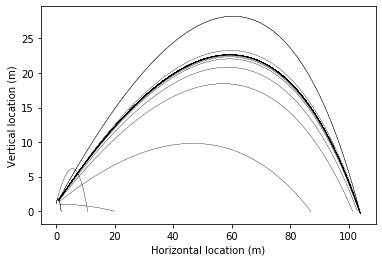
\includegraphics[scale=0.6]{src/4.4 constrained ball optimisation.png}
    \caption{Constrained ball optimisation graph.}
\end{figure}
\noindent The optimised throw angle is $32.4^{\circ}$ and strength $1.00$, with distance $104.0$ m. Instead, if we used a penalty term to optimise, the penalty function could be the following.
\begin{figure}[H]
    \centering
    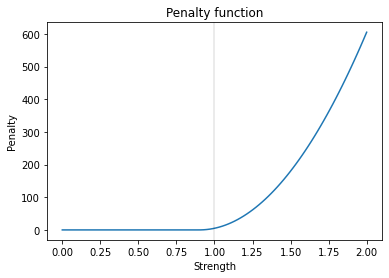
\includegraphics[scale=0.6]{src/4.5 penalty function.png}
    \caption{The penalty function.}
\end{figure}
\noindent We want to discourage solutions that exceed strength value of 1, so the penalty function increases exponentially after 1. This gives us the following graph of solutions:
\begin{figure}[H]
    \centering
    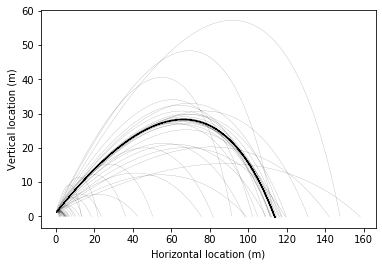
\includegraphics[scale=0.7]{src/4.6 penalty ball optimisation.png}
    \caption{The penalty ball optimisation graph.}
\end{figure}
\noindent The optimised throw angle is $35.2^{\circ}$ and strength $1.06$, with distance $101.1$ m.

\section{Properties of the objective function}
\subsection{Convexity: global and local minima}
An objective function can have a local minima. A local minimum is a point where the function is increasing in every direction from that point. If the function is convex, then there is precisely one global minimum. For example, the following functions are convex.
\begin{figure}[H]
    \centering
    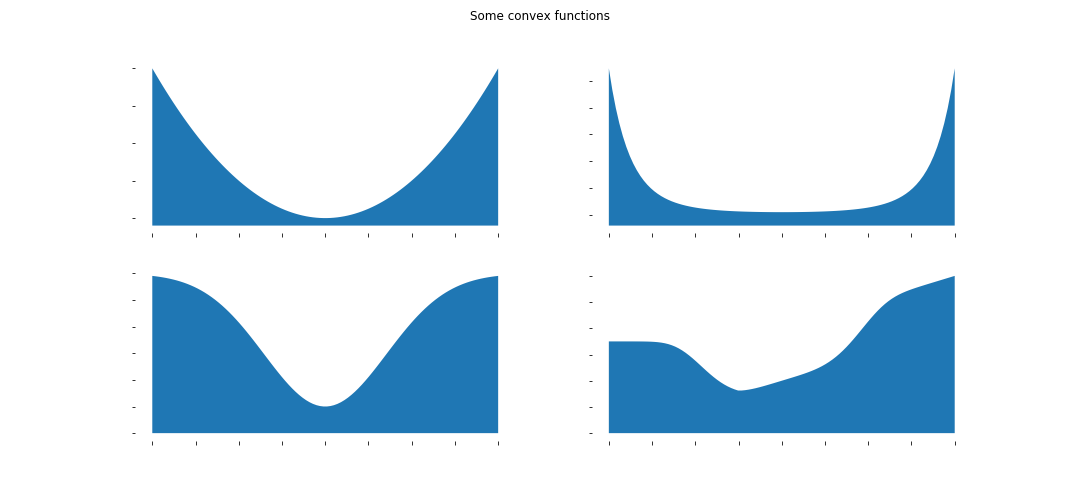
\includegraphics[scale=0.315]{src/4.7 convex functions.png}
    \caption{Convex functions.}
\end{figure}
\noindent Other functions can have multiple local minima, i.e. there could be some local minimum that is not the optimal value (not the global minimum). For example, the following functions are not convex.
\begin{figure}[H]
    \centering
    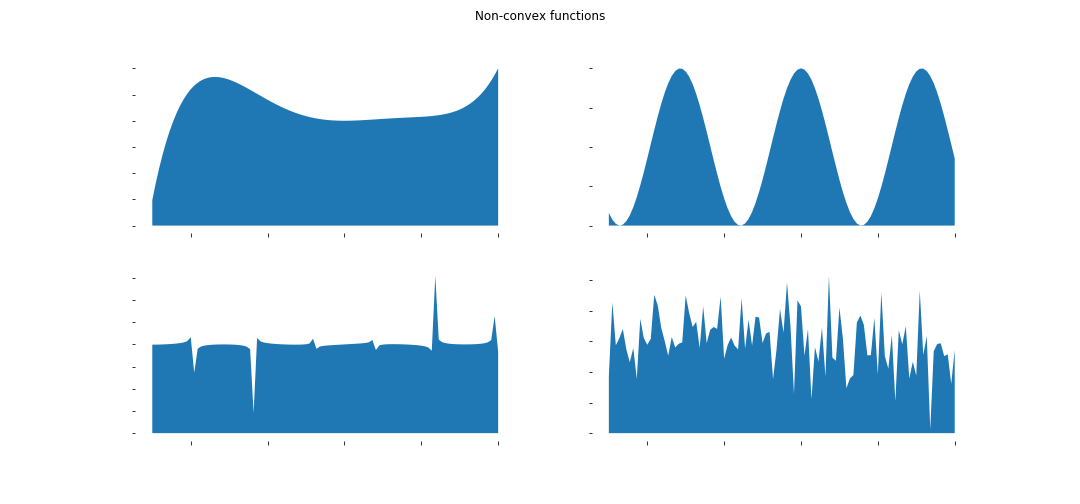
\includegraphics[scale=0.315]{src/4.8 nonconvex functions.png}
    \caption{Non-convex functions.}
\end{figure}

If the objective function that is convex and the constraints form a convex portion of the search space, then the problem is called convex optimisation. These can be solved very optimally, even if they have hundreds of variables. These include:
\begin{itemize}
    \item linear programming, i.e. the constraint and the objective function are linear;
    \item quadratic programming, i.e. the objective function is quadratic, and the constraint linear; and
    \item some other special cases, e.g. semi-quadratic programming, quadratically constrained quadratic program.
\end{itemize}
For non-convex functions, we typically use some iterative method to optimise. It is also possible to relax/approximate a function into some convex function.

\subsection{Continuity}
An objective function is continuous if small changes in $\theta$ lead to small changes in $L(\theta)$. In other words, there are no jumps in the function. For example, the following function is continuous.
\begin{figure}[H]
    \centering
    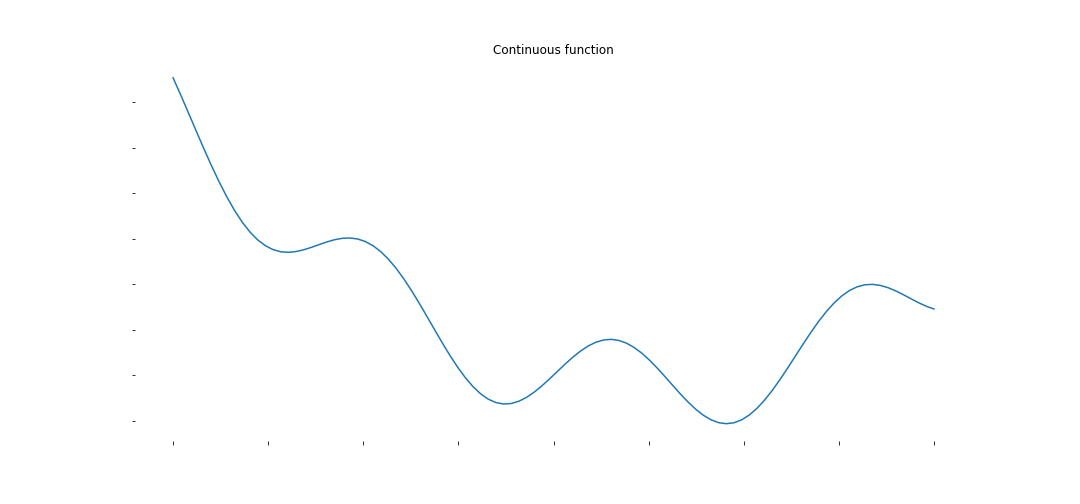
\includegraphics[scale=0.3]{src/4.9 continuous functions.png}
    \caption{A continuous function.}
\end{figure}
\noindent If the function is discontinuous, local search methods need not converge to a solution. For example, the following function is discontinuous.
\begin{figure}[H]
    \centering
    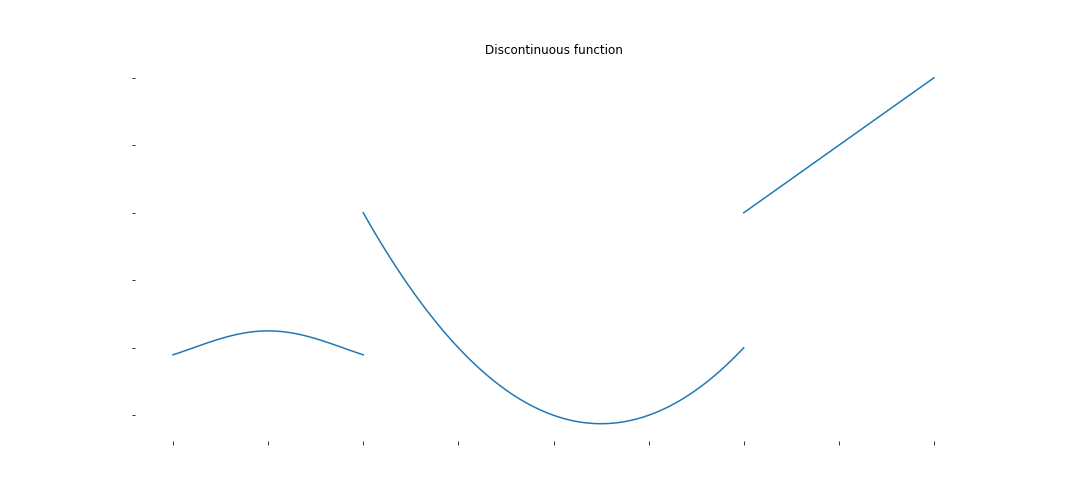
\includegraphics[scale=0.3]{src/4.10 noncontinuous functions.png}
    \caption{A discontinuous function.}
\end{figure}
\noindent Optimising discontinuous objective functions is typically much harder than optimising continuous function- small changes in the parameter can lead to arbitrary changes in the objective function. Continuity is why continuous optimisation is easier than discrete optimisation.

\section{Algorithms}
\subsection{Linear Least Squares}
The linear least squares is an optimisation technique which tries to find the closest set of parameters $\mathbf{x}$ such that $A \mathbf{x}$ is as close to $\mathbf{y}$ as we can. So, the objective function is
\[L(\mathbf{x}) = \lVert A \mathbf{x} - \mathbf{y} \rVert_2.\]
This equation is convex- the function is quadratic, so it must have one global minimum (even if $\mathbf{x}$ has multiple dimensions). Quadratic functions have either one or zero minimum.

\subsection{Line fitting}
Given a pair of vectors $\mathbf{x}$ and $\mathbf{y}$, we can try to fit a line through it. We saw in the previous chapter that we can use pseudo-inverse (via SVD) to fit a line. We will create samples from $y = 2x + 1$ with some noise. Usng the SVD, we get the following estimate:
\begin{figure}[H]
    \centering
    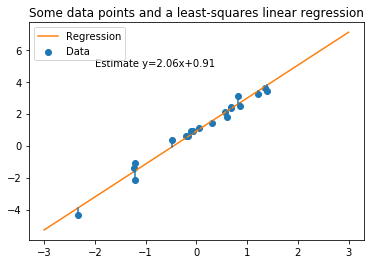
\includegraphics[scale=0.6]{src/4.11 linear regression least squares.png}
    \caption{Linear regression using least squares.}
\end{figure}

\subsection{Iterative optimisation}
An iterative optimisation takes a series of steps in the parameter space to find the local minimum, until the terminating criterion is met. There is a current parameter (or a collection of them). The algorithm essentially involves:
\begin{verbatim}
choose a starting point x0;
while the objective function is changing:
    adjust parameters;
    evaluate the objective function;
    if better solution found, change the best parameter;
return the best parameter;
\end{verbatim}

\subsection{Grid Search}
Grid search is a simple yet ineffective optimisation for multidimensional problems. We sample the parameter space by breaking it into equally divided grids, usually with a fixed number of divisions per dimension. The objective is function is evaluated at each $\theta$ on this grid, and we keep track of the lowest $\theta$. It is sometimes used to optimise hyperparameters, where the objective function may be complex but the absolute minimum isn't essential.

The following image illustrates the grid search algorithm to find the line fit through the data above.
\begin{figure}[H]
    \centering
    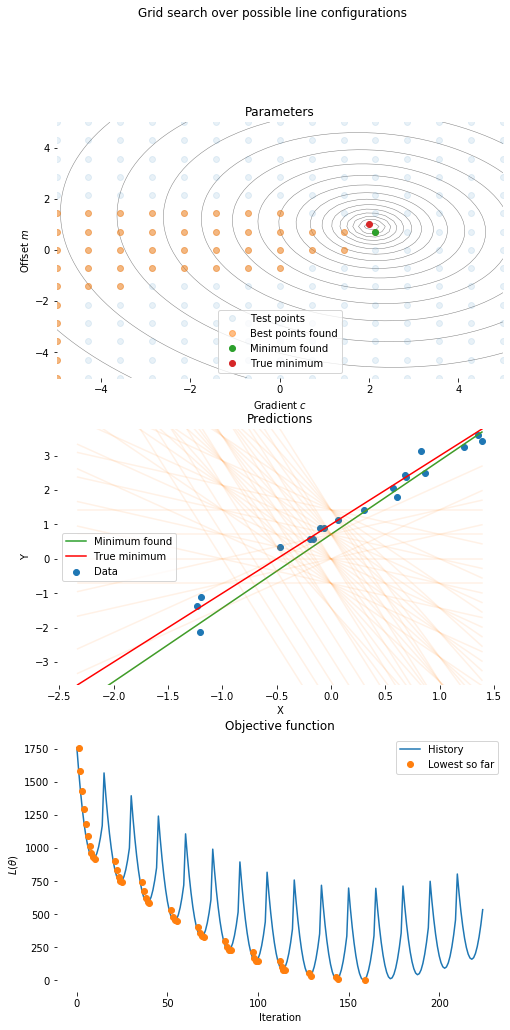
\includegraphics[scale=0.5]{src/4.12 grid search line configurations.png}
    \caption{Grid search line configurations.}
\end{figure}
The reason grid search is inefficient at optimisation in higher dimensions is the curse of dimensionality. If we want to break a grid into 8 portions, in 1D, this would be 8 blocks; in 2D, this would be 64 blocks; and so on. The following figure describes how the grids are positioned:
\begin{figure}[H]
    \centering
    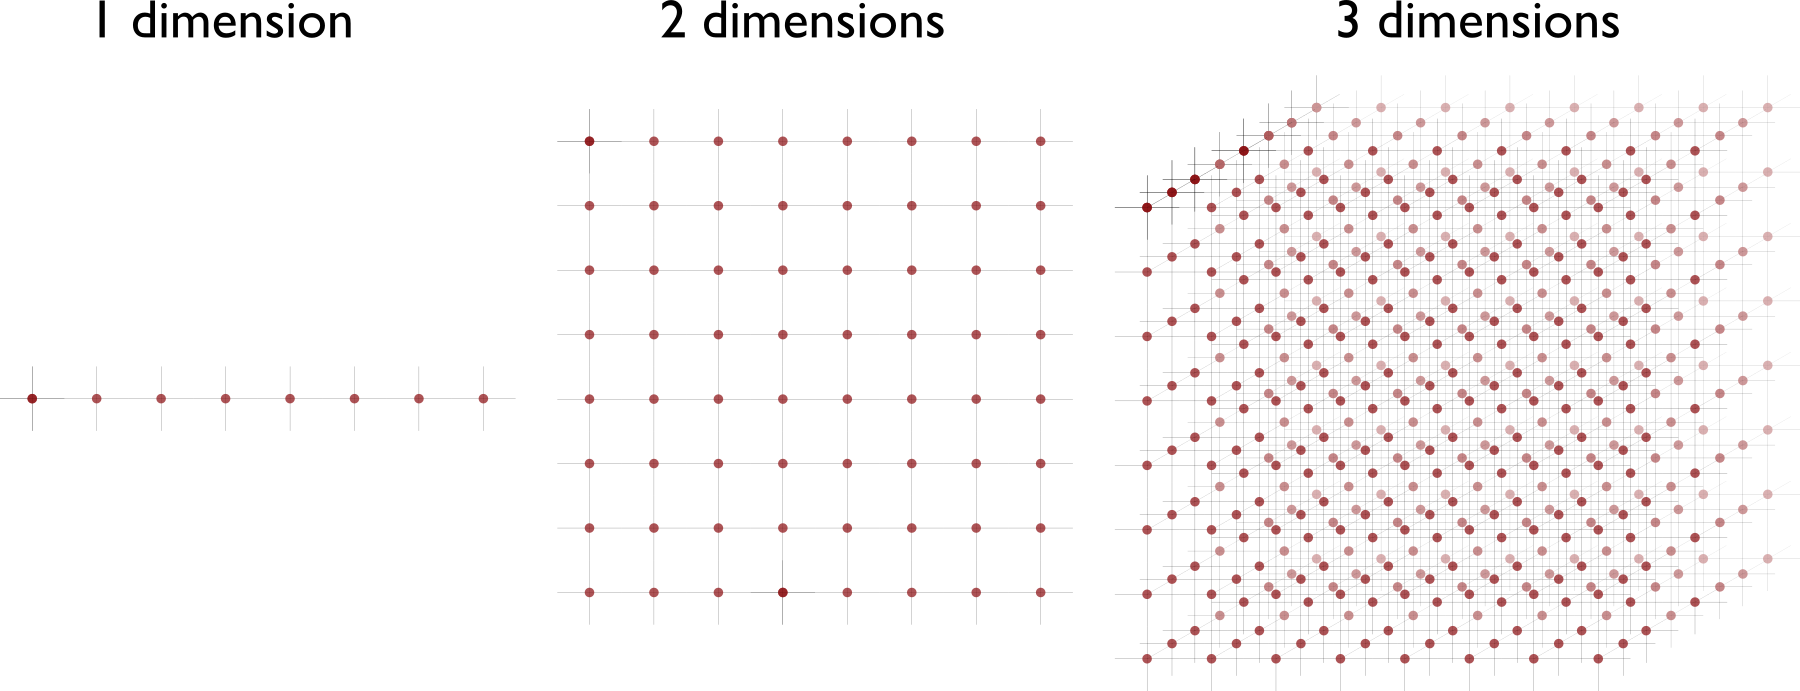
\includegraphics[scale=0.3]{src/4.13 grid search dimensions.png}
    \caption{Grid search dimensions.}
\end{figure}
\noindent In 100D, this would be $8^{100} \approx 2.04 \times 10^{89}$ blocks- we would need to evaluate the function that many times. Even with 3 portions is infeasible ($3^{100} \approx 5.15 \times 10^{46}$). Moreover, if the objective function isn't very smooth, the grid would need to be very dense to find the optimsation configuration. The following figure describes how the minimum is missed during the grid search because of the way the grid has been divided.
\begin{figure}[H]
    \centering
    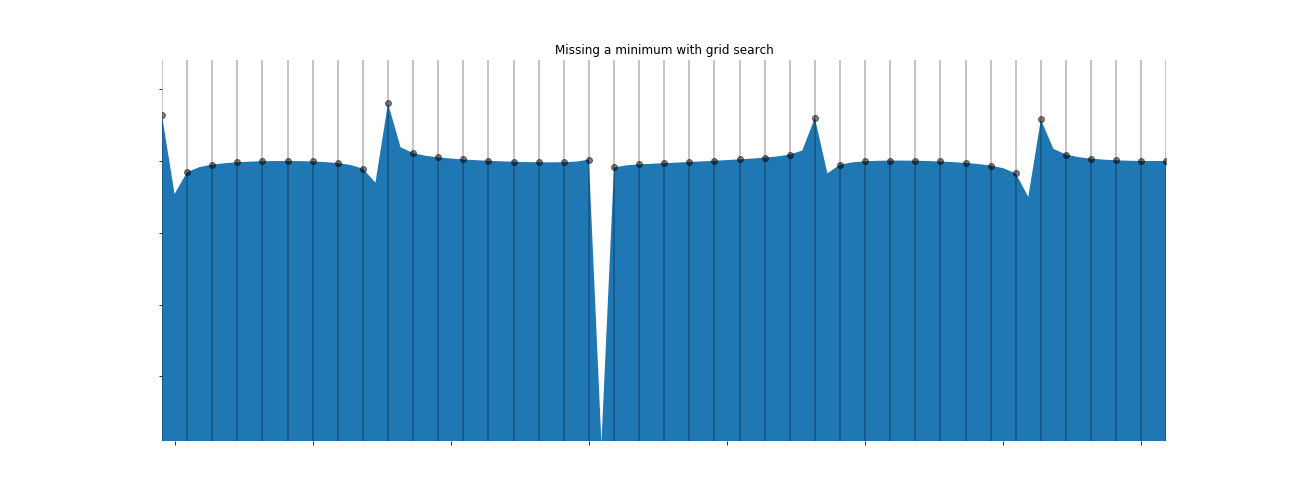
\includegraphics[scale=0.25]{src/4.14 density of grid search.png}
    \caption{Missing a minimum with grid search.}
\end{figure}
The pros of grid searching are:
\begin{itemize}
    \item works for any continuous parameter space;
    \item requires no knowledge of the objective function (it need not even be continuous); and
    \item trivial to implement.
\end{itemize}
The cons of grid searching are:
\begin{itemize}
    \item incredibly inefficient;
    \item must specify the search space bounds in advance;
    \item highly biased to finding things near the ``early corners'' of the space;
    \item depends heavily on the number of divisions chosen; and
    \item hard to tune so that the minima aren't missed entirely.
\end{itemize}

\subsection{Hyperparameters}
Grid search depends on how we partition the grid. Most optimisation algorithms have some parameters that can be tweaked and affect the efficiency of the algorithm. The properties that affect how an optimiser can find the solution are called hyperparameters. They are not parameters of the objective function, but they affect the results obtained. We would like to have few (if any) hyperparameters.

\subsection{Random search}
The simplest optimisation is random searching. The algorithm randomly samples the parameter space and then returns the parameter that minimises the loss function. Essentially:
\begin{itemize}
    \item guess a random parameter $\theta$;
    \item check the objective function $L(\theta)$;
    \item if better than the previous parameter, change to this one.
\end{itemize}
There are many possible termination conditions, e.g. certain number of iterations.

The pros of random search is:
\begin{itemize}
    \item cannot get trapped in a local minimum (as there is no structure in the algorithm);
    \item requires no knowledge of the objective function (not even a topology);
    \item very simple to implement;
    \item better than grid search almost always.
\end{itemize}
The cons of random search is:
\begin{itemize}
    \item extremely inefficient, and only appropriate if there is no structure in data to exploit;
    \item must be possible to random sample the parameter space;
    \item results do not necessarily get better, i.e. there is no way to predict how the optimisation would proceed.
\end{itemize}

The following figure illustrates the random search algorithm to find the line fit through the data above.
\begin{figure}[H]
    \centering
    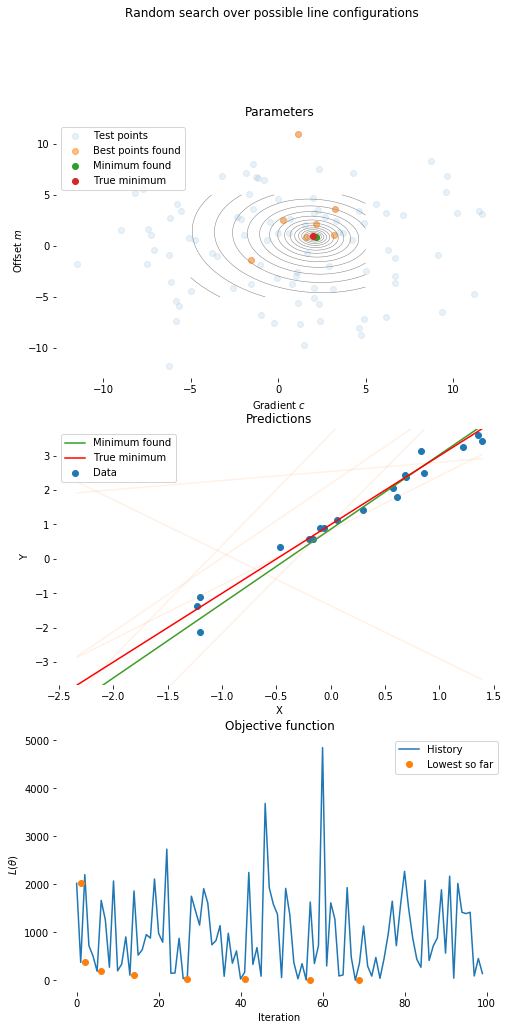
\includegraphics[scale=0.5]{src/4.15 random search line configurations.png}
    \caption{Random search line configurations.}
\end{figure}

\section{Metaheuristics}
We can use metaheuristics to improve random searching.
\begin{itemize}
    \item Locality: if the objective function is continuous, changing the parameters slightly will only change the value of the objective function slightly;
    \item Temperature: we can change the rate of movmeent on the parameter space as the optimisation proceeds, assuming that there exists a local minimum;
    \item Population: we can keep track of multiple parameter configurations at the same time, and mix them around to combine the best of both sets;
    \item Memory: we can keep track of good and bad steps we took and try avoid/revisiting them.
\end{itemize}

\subsection{Locality}
Local searching algorithms make incremental changes towards a local minimum. If the function is continuous, these are much more efficient than random/grid searching. But, since they only find local minima, there is no guarantee that the minima is global, i.e. there might be a smaller value the function attains, but the iterative algorithm must have gotten stuck in another, bigger local minima. 

The local minima we find depends on the initial conditions. Local searching creates a trajectory through the parameter space such that the objective function is getting smaller. The following graph illustrates these two points.
\begin{figure}[H]
    \centering
    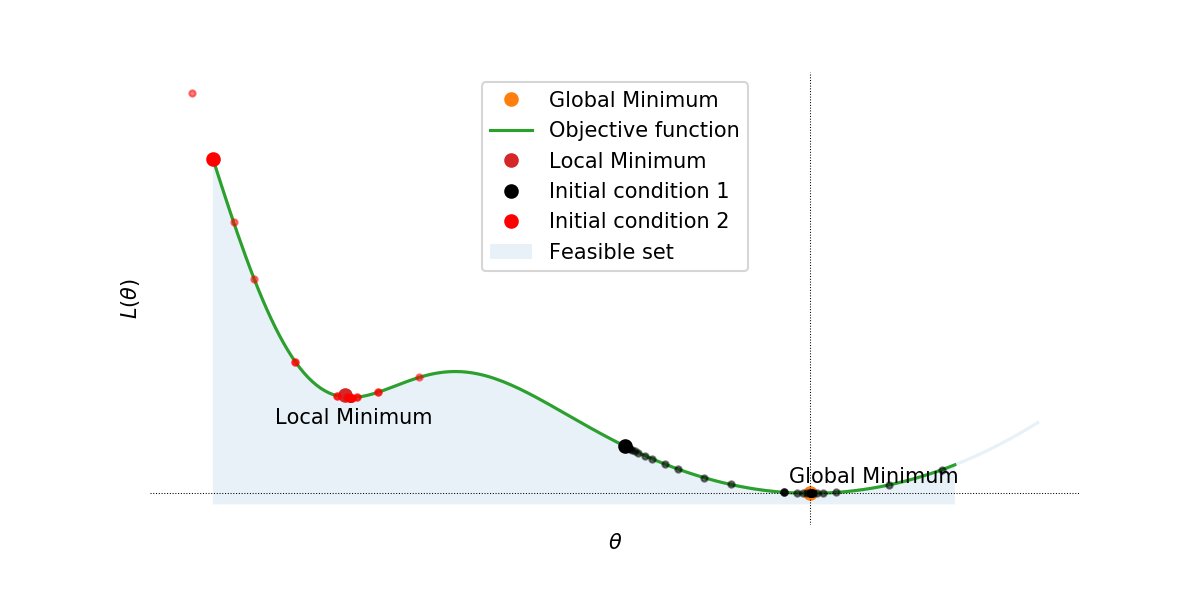
\includegraphics[scale=0.5]{src/4.16 locality.png}
    \caption{How the local mimum depends on the initial condition.}
\end{figure}

A local searching algorithm is hill climbing. It modifies the random searching algorithm and assumes some topology of the parameter space so we can find a neighbourhood around the parameter vector. This allows us to make incremental changes to it. Instead of drawing random samples, we sample near the current best parameter in hopes of finding an even more optimal configuration. We only change the parameter given that the loss function gets smaller.

Simple hill climbing only changes one of the parameter vector elements in one go, examining each direction in turn. Stochastic hill climbing makes a random change to the parameter vector (i.e. all the components get changed). It either accepts or rejects the change depending on whether the loss function get smaller.

The following figure illustrates the hill search algorithm to find the line fit through the data above.
\begin{figure}[H]
    \centering
    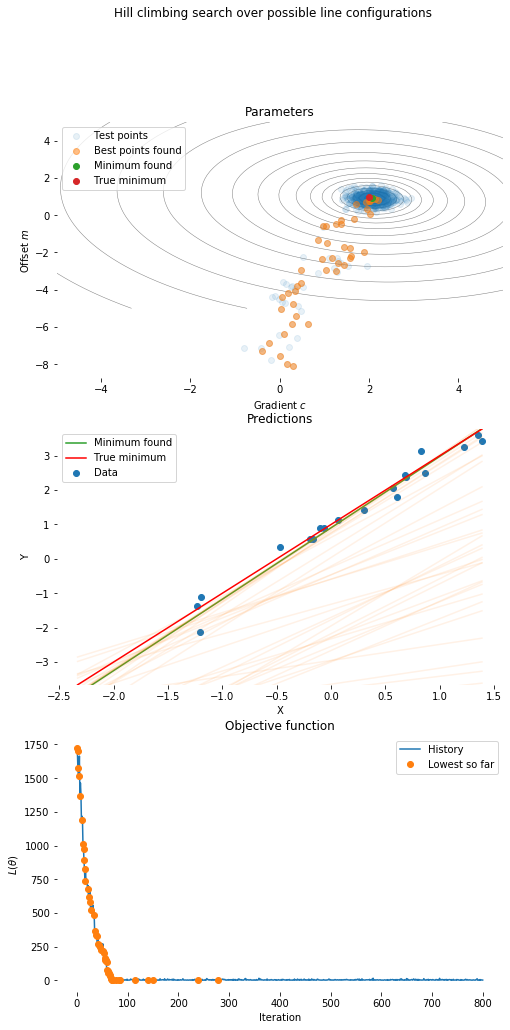
\includegraphics[scale=0.5]{src/4.17 hill climbing search line configurations.png}
    \caption{Hill climbing search line configurations.}
\end{figure}

The pros of hill climbing are:
\begin{itemize}
    \item not much more complicated than random searching;
    \item can be much faster than random searching.
\end{itemize}
The cons of hill climbing are:
\begin{itemize}
    \item hard to choose how much of an adjustment to make;
    \item can get stuck in a local, non-global minimum;
    \item struggles with objective functions that are relatively flat;
    \item requires the function to be (mostly) continuous.
\end{itemize}

We can tweak the algorithm to improve it. We can use adaptive local search- the size of the neighbourhood can be adapted, e.g. if there was no improvement made for some number of iterations. Also, we can use multiple restart- we start at different positions to avoid getting stuck at a local minimum (this is another metaheuristic- a heuristic applied to the algorithm itself).

\subsection{Temperature}
Simulated annealing extends hill climbing with the ability to make bad choices (go uphill) instead of always making good choices (go downhill). This is to help overcome ridges and getting stuck at a local minimum.

The following is a possible simulated annealing temperature schedule.
\begin{figure}[H]
    \centering
    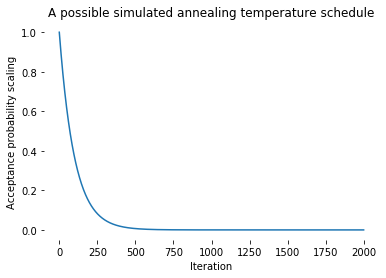
\includegraphics[scale=0.7]{src/4.18 a possible simulated annealing temperature schedule.png}
    \caption{A possible simulated annealing temperature schedule.}
\end{figure}
\noindent The following figure illustrates the simulated annealing algorithm to find the line fit through the data above, using the temperature schedule above.
\begin{figure}[H]
    \centering
    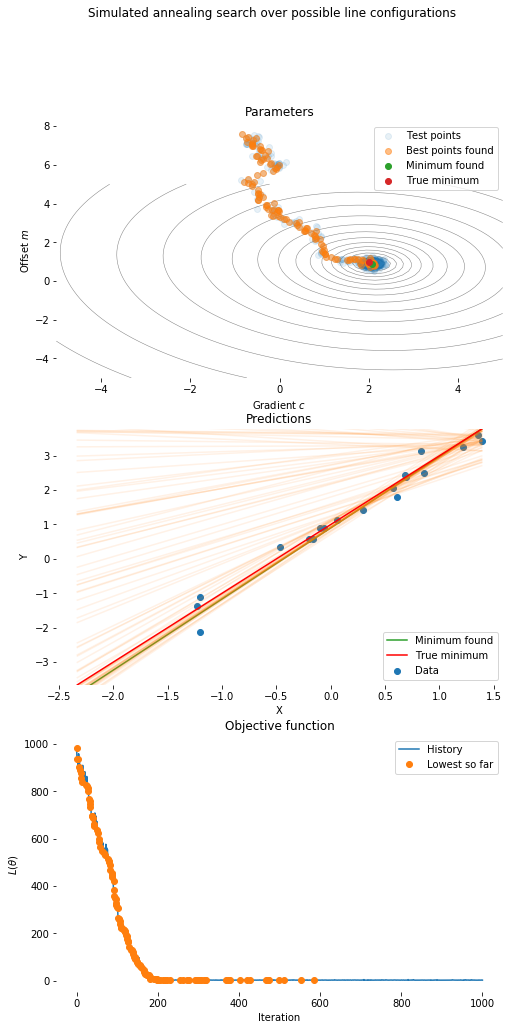
\includegraphics[scale=0.5]{src/4.19 simulated annealing search line configurations.png}
    \caption{Simulated annealing search line configurations.}
\end{figure}


\subsection{Population}
We can apply an analogue of evolution in optimisation, by:
\begin{itemize}
    \item mutating, i.e. introducing random variation;
    \item natural selection, i.e. solution selection; and
    \item breeding, i.e. interchange between solutions.
\end{itemize}
Algorithms that use these techniques are called genetic algorithms. These algorithms maintain a population of potential solutions, and some rule to preserve some and to cull the others. The parameter set is called the genotype of a solution.

A simple selection rule would be: keep the 25\% solutions, ordered by loss. Each iteration would add some mutation, cull the weakest solutions, copy the remaining solutions a number of times to produce the offspring for the next step. The size of the population is constant during each iteration. Using this, we can explore a large area of the space than a simple local search.

More advanced algorithms introduce some form of breeding or crossover. In crossover, two (or more) parameter vectors are merged to give a child parameter vector. Crossover works well when the parameter space can be partitioned into multiple components, so that the offspring can inherit good qualities from the parents. It works less well when the crossover simply becomes a mismatch of parent qualities that average out.

The pros of genetic algorithms are:
\begin{itemize}
    \item Easy to understand and applicable to many problems;
    \item Requires only weak knowledge of the objective function;
    \item Can be applied to problems with both discrete and continuous components;
    \item Some robustness against local minima, although hard to control and guarantee;
    \item Great flexibility in parametrisation such as mutation schemes, crossover schemes, fitness functions, selection functions, etc.
\end{itemize}
The cons of genetic algorithms are:
\begin{itemize}
    \item Many hyperparameters that affect the performance of the optimisation;
    \item No guarantee of convergence;
    \item Very slow compared to using stronger knowledge of the objective function;
    \item Many evaluations of the objective function required: one per population member per iteration.
\end{itemize}

The following figure illustrates the genetic algorithm to find the line fit through the data above.
\begin{figure}[H]
    \centering
    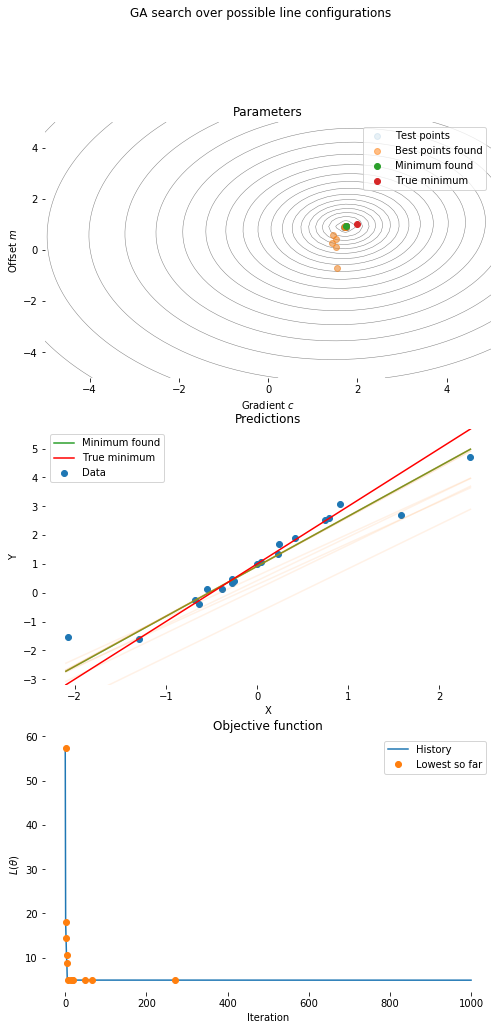
\includegraphics[scale=0.5]{src/4.20 genetic algorithm line configurations.png}
    \caption{Genetic algorithm line configurations.}
\end{figure}

\subsection{Memory}
The optimisation algorithms we have seen have had no memory- they do not keep track of the points hat gave us a bad loss value. For this reason, they might check the same/similar values again and again. We can use some memory, where the optimiser remembers good and bad bits of the paraameter space, especially the good paths in the solution space. We want to have a population of parameter sets, and a memory of good paths through the space.

The pros of memory algorithms are:
\begin{itemize}
    \item can be very good when solutions are separated by large, narrow valleys;
    \item can have fewer evaluations of the objective function that genetic algorithms if paths are effective;
    \item when it works, it really works.
\end{itemize}
The cons of memory algorithms are:
\begin{itemize}
    \item moderately complex algorithm to implement;
    \item no guarantee of convergence;
    \item even more hyperparameters than genetic algorithms.
\end{itemize}

\section{Quality of optimisation}
\subsection{Convergence}
We say that an optimisation algorithm converges to a solution. In convex optimisation, we find the global maximum and the problem is solved. In non-convex optimisation, we have found a local maximum and are stuck.

A good optimisation algorithm converges quickly. This means that the objective function drops steeply- each iteration makes a big difference. A bad optimisation algorithm does not converge at all (it wonders forever, or diverges to infinity). We compare the convergence of the algorithms we saw above in solving the linear regression problem above.
\begin{figure}[H]
    \centering
    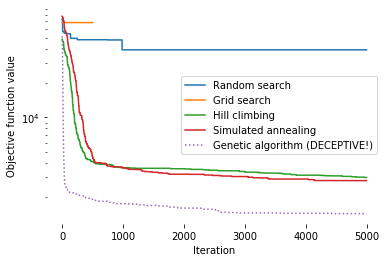
\includegraphics[scale=0.6]{src/4.21 search comparisons.png}
\end{figure}

Most optimisation algorithms only convergence in the right conditions. The convergence depends on the initial conditions of the optimisation. Some algorithms are guaranteed to converge if a solution exists, while others (most heuristic optimisation algorithms) are not guaranteed to converge even if there is a solution. For iterative algorithms, it is possible to plot how the objective function is decreasing as the iteration proceeds to determine convergence problems. Ideally, the loss should drop as fast as possible.

\subsection{Tuning optimisation}
To use optimisation algorithms efficiently, we need to tune its hyperparameters. If we know the problem is of specific sort, then we should use the algorithm that converges the best for it, e.g.
\begin{itemize}
    \item if the problem is least-squares, use a least-squares solver (it might even be possible to solve it directly using pseudo-inverse);
    \item if the problem is convex, use a convex solver (a convex solver is much more efficient than a normal solver);
    \item if the problem is differentiable, use a first-order method; and
    \item if none of these is known, use a genetic algorithm or simulated annealing.
\end{itemize}

Many things could go wrong, such as:
\begin{itemize}
    \item The algorithm might make slow process. This can happen in local searching if the step size is too small, e.g. in gradient descent, a small step size $\delta$ would only change the objective function by little, which means that we are only searching a small portion of the space. We illustrate how step size affects convergence in hill climbing.
    \begin{figure}[H]
        \centering
        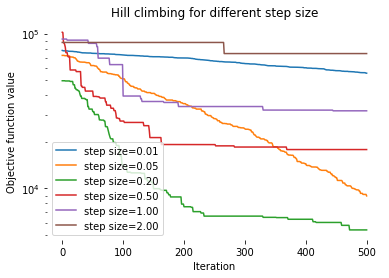
\includegraphics[scale=0.6]{src/4.22 hill climbing for different step size.png}
        \caption{Hill climbing for different step sizes}
    \end{figure}
    
    \item The algorithm may have noisy and divergent performance. Local searching can become unstable, especially if the jumps are too large, or if the objective function is infinitely ddecreasing (we would need to constraint the parameter space in that case).
    
    \item The algorithm might get stuck at critical points of the functions, e.g.
    \begin{itemize}
        \item plateaus (a neighbourhood where the function is constant)- a memoryless algorithm might wander around, and a derivative-based one gets stuck. We can use momentum and other forms of memory to limit this effect.
        \item local minima- local searching can get trapped in local minima. We can use random restart to limit this effect.
        \item saddle points (the function is increasing in one direction, and decreasing in some other direction)- this can slow or trap gradient descent methods since it will have a hard time trying to find the best direction to travel.
        \item very steep/discontinuous- this can produce huge barriers for gradient descent. Stochastic gradient descent can blur out these boundaries and still make progress.
    \end{itemize}
    The image below summarises the different kinds of critical points.
    \begin{figure}[H]
        \centering
        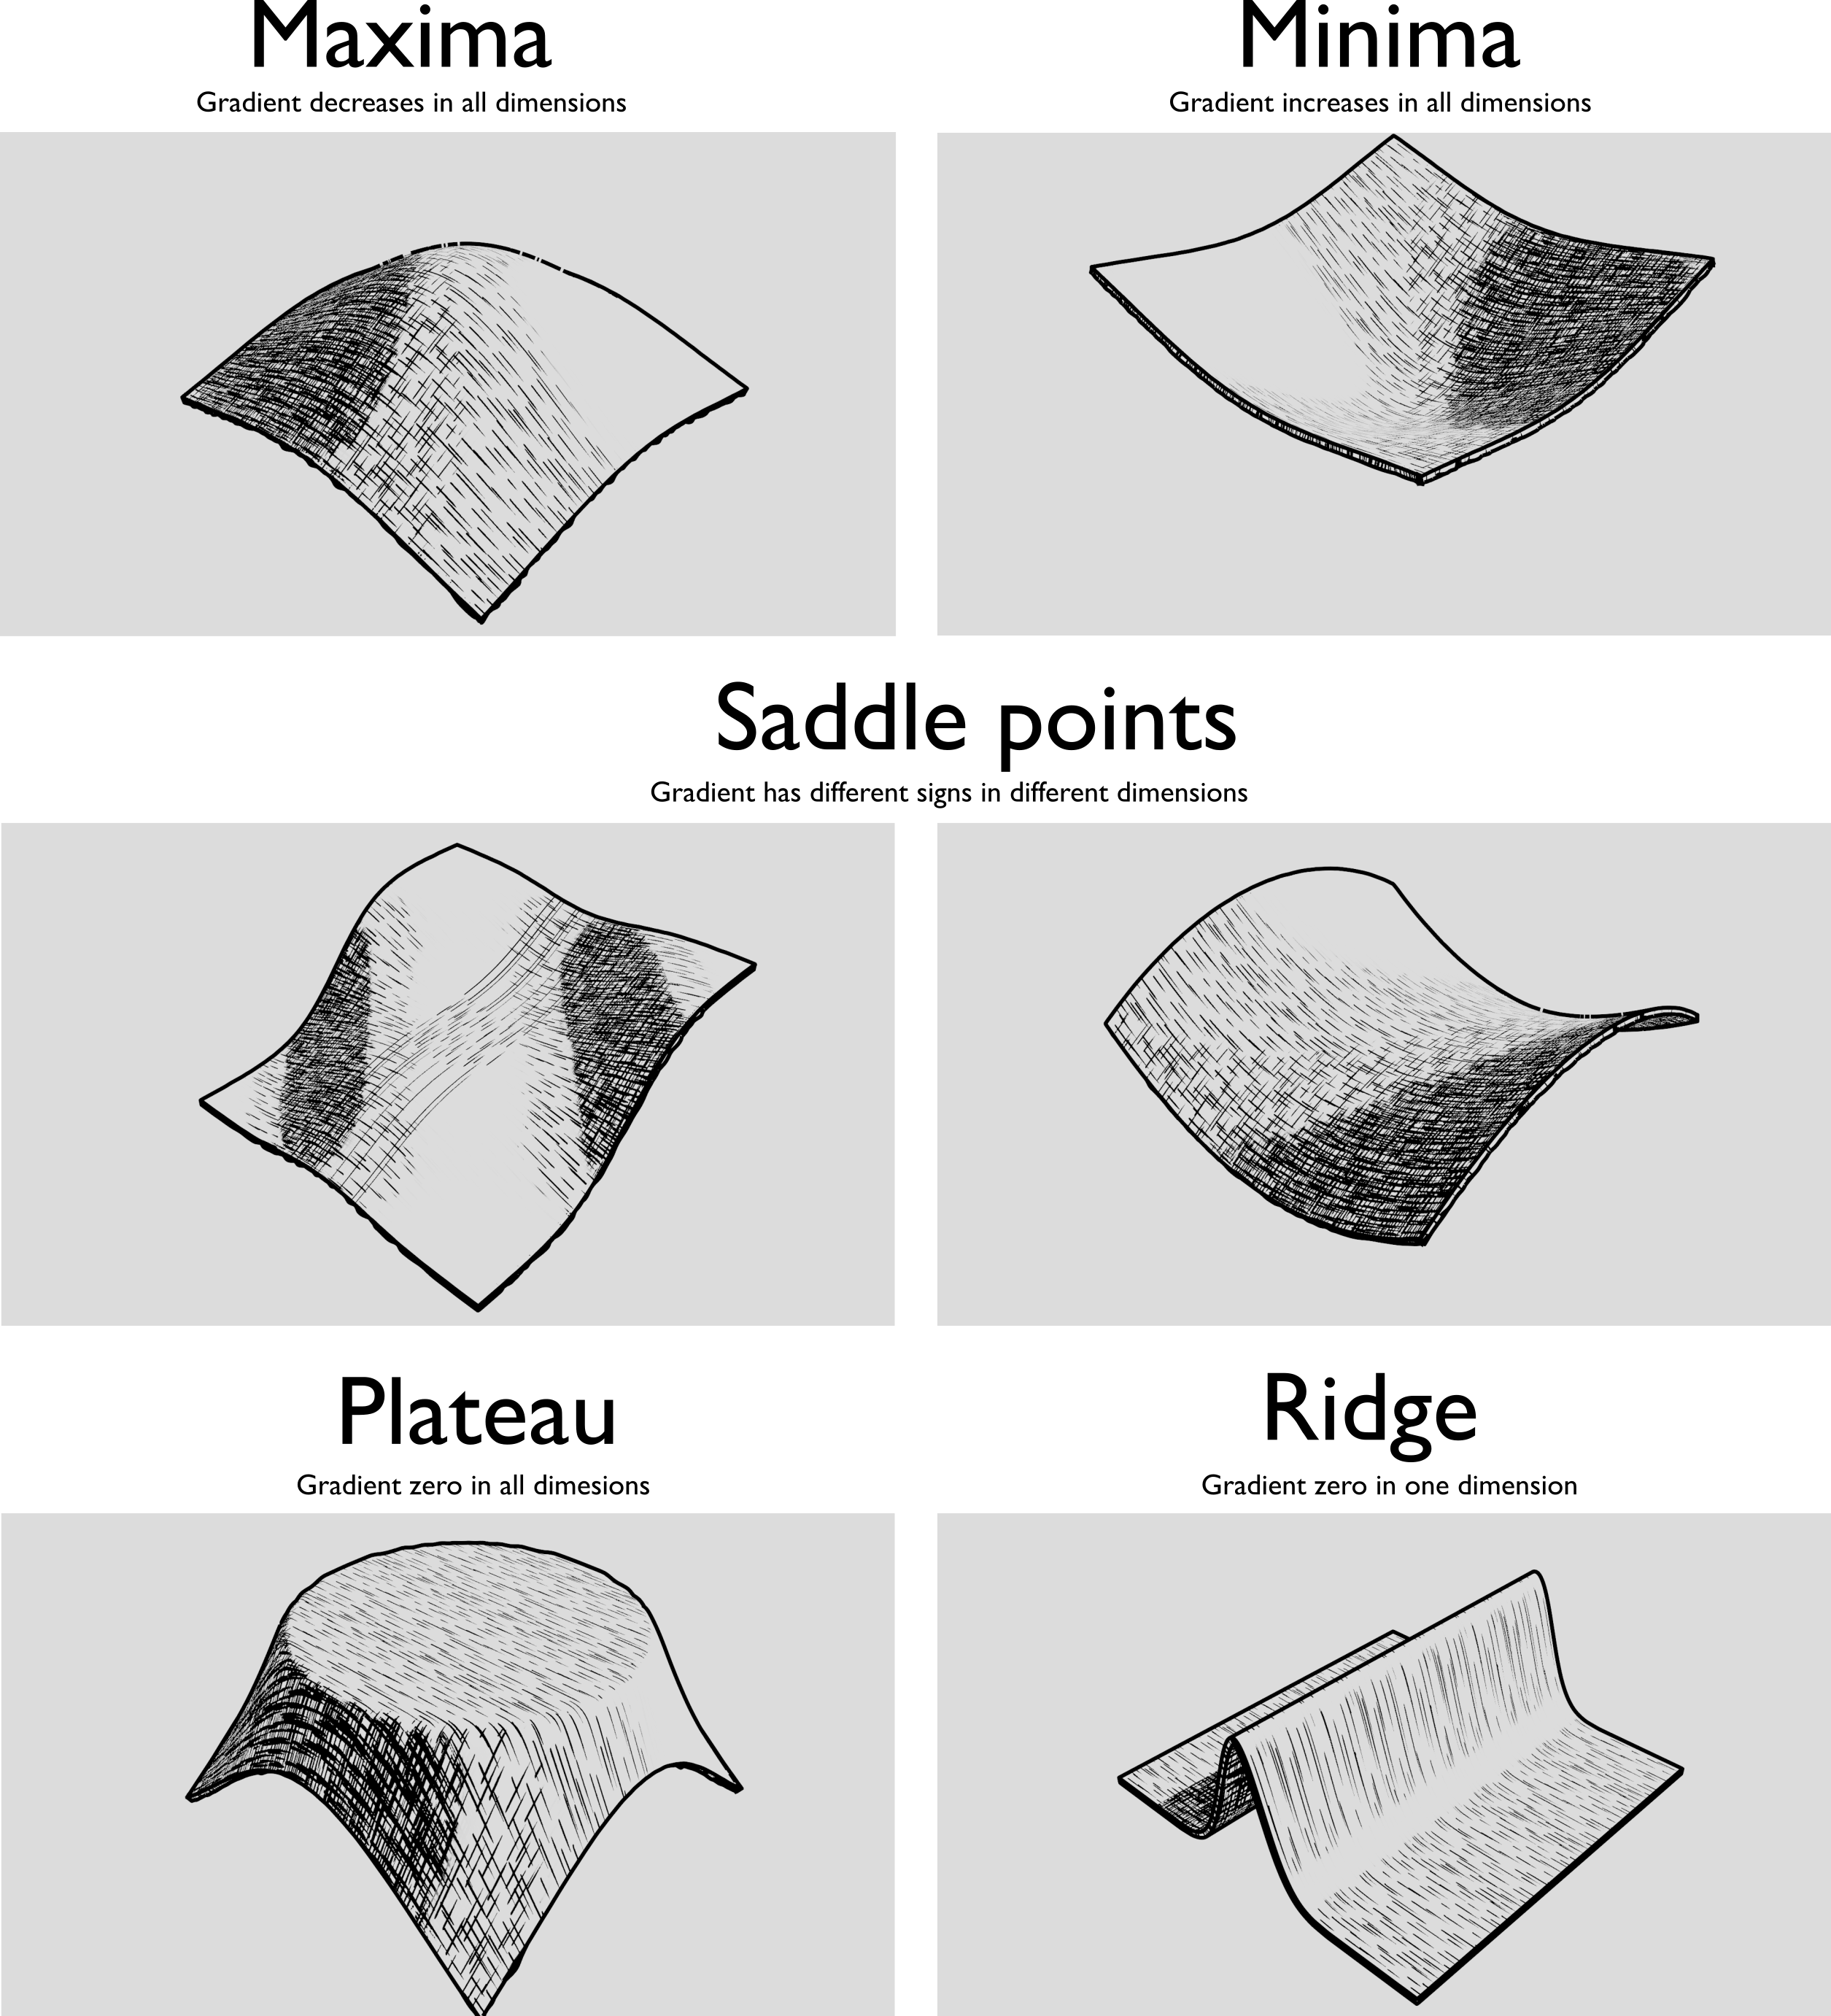
\includegraphics[scale=0.15]{src/4.23 2D stationary points.png}
        \caption{Critical points in $\mathbb{R}^2$.}
    \end{figure}
\end{itemize}

\section{Deep Neural Networks}
Deep learning or deep neural networks have become a major part of modern machine learning research. They have had astonishing success in fields like speech recognition, machine translation, image classifcation and image synthesis.

In deep learning, we essentially aim to approximate a given function. For instance, we might be given a set of observations $\mathbf{x}_1, \mathbf{x}_2, \dots, \mathbf{x}_n$ and corresponding outputs $\mathbf{y}_1, \mathbf{y}_2, \dots, \mathbf{y}_n$, and we want to find a function $\mathbf{y}' = f(\mathbf{x}, \theta)$ where $\mathbf{x}$ is some observation and $\theta$ a set of parameters, such that
\[\theta^* = \operatornamewithlimits{argmin}_\theta \sum_i \lVert f(\mathbf{x}_i, \theta) - \mathbf{y}_i \rVert.\]
We can then use the function $f$ to predict outputs for unseen observations. Clearly, it is an optimisation problem. The difficult here is that we can have millions of parameters, so we need to come up with a way to optimise in such a large vector space in a reasonable amount of time.

The way we deal with this is that the networks are constructure in a simple way. A neural network typically consists of layers, each of which is a linear map followed by a simple, fixed, non-linear function. It is like: rotate, stretch (linear map) and fold (simple non-linear folding). The output of one layer is the input of the next layer.

The linear map in each layer is specified by a matrix (a weight matrix). The network is completely parameterised by the entries of the weight matrices for each layer (all of the entries of these matrices can be seen as the parameter vector $\theta$). The nonlinear function $G(x)$ is fixed for each layer and cannot vary.

The reason this is efficient is that the derivative of the objective function with respect to the weights can be computed for every weight in the network at the same time. This is called backpropagation, and it is an algorithm for automatic difference.

\subsection{Heuristic searching}
Heuristic searching methods are easy to understand and implement, and works in most cases. However,
\begin{itemize}
    \item it can be very slow. It acn take many iterations to approach a minimum and require significant computation to compute each iteration.
    \item there is no guarantee of convergence (or even progress). The search can get stuck, or drift away over plateaus.
    \item there are a lot of hyperparameters that can be tweaked (temperature schedules, size of population, memory structure, etc.). Optimal choice of these parameters becomes an optimisation problem in itself.
\end{itemize}

For optimisation problems like deep neural networks, heuristic search is inadequate. It is simply too slow to make progress in training networks with millions of parameters. Instead, first-order optimisation is applied. First-order algorithms can be orders of magnitude faster than heuristic search.

\subsection{Rolling a ball}
An intuition for higher-order optimisation can be formed by considering a ball rolling on a (smooth) surface, which represents the value of the objective function across a 2D domain (i.e. if we had a parameter vector $\theta$ with two elements). The ball will eventually settle in a configuration where there is a balanced set of forces applied to it. This will happen, for example, if the ball settles at a minimum where the normal of the surface is parallel with gravity.

\section{Derivatives}
If the function $f$ is a scalar function, then $f'(x) = \frac{dy}{dx}$ is the first derivative with respect to $x$. The second derivative with respect to $x$ is $f''(x) = \frac{d^2 y}{dx^2}$. In general, if the function $f$ maps to $\mathbb{R}^n$, then we have an $n \times n$ derivative matrix, called the Jacobian, i.e.
\[f'(\mathbf{x}) = \begin{bmatrix}
    \frac{\partial y_0}{\partial x_0} & \frac{\partial y_0}{\partial x_1} & \dots & \frac{\partial y_0}{\partial x_n} \\
    \frac{\partial y_0}{\partial x_0} & \frac{\partial y_1}{\partial x_1} & \dots & \frac{\partial y_1}{\partial x_n} \\
    \vdots & \vdots & \ddots & \vdots \\
    \frac{\partial y_0}{\partial x_0} & \frac{\partial y_n}{\partial x_1} & \dots & \frac{\partial y_n}{\partial x_n} 
\end{bmatrix}.\]

The gradient vector for the function is one row of the Jacobian matrix. It tells us how $f$ would vary as we change one of the parameters with respect to each dimension, separately. We will only consider functions going from $\mathbb{R}^n$ to $\mathbb{R}$. So,
\[\nabla L(\theta) = \begin{bmatrix}
    \frac{\partial L(\theta)}{\partial \theta_1} & \frac{\partial L(\theta)}{\partial \theta_2} & \dots & \frac{\partial L(\theta)}{\partial \theta_n} 
\end{bmatrix}.\]
If $L(\theta)$ is a map $\mathbb{R}^n$ to $\mathbb{R}$, then $\nabla L(\theta)$ is a map $\mathbb{R}^n \to \mathbb{R}^n$. If $L(\theta)$ is a map $\mathbb{R}^n \to \mathbb{R}^m$, then $\nabla L(\theta)$ is a map $\mathbb{R}^n \to \mathbb{R}^{m \times n}$.

The Hessian matrix is the Jacobian of a gradient vector, denoted by $\nabla^2 f(\mathbf{x})$. It is equivalent to the second derivative for vector functions. The function $\nabla^2 L(\theta)$ is a map $\mathbb{R}^n \to \mathbb{R}^{n \times n}$. In particular,
\[H(L) = \nabla^2 L(\theta) = \begin{bmatrix}
    \frac{\partial^2 L(\theta)}{\partial \theta_1^2} & \dots & \frac{\partial^2 L(\theta)}{\partial \theta_1 \partial \theta_{n-1}} & \frac{\partial^2 L(\theta)}{\partial \theta_1 \partial \theta_n} \\
    \frac{\partial^2 L(\theta)}{\partial \theta_2 \partial \theta_1} & \dots & \frac{\partial^2 L(\theta)}{\partial \theta_2 \partial \theta_{n-1}} & \frac{\partial^2 L(\theta)}{\partial \theta_2 \partial \theta_n} \\
    \vdots & \vdots & \ddots & \vdots \\
    \frac{\partial^2 L(\theta)}{\partial \theta_n \theta_1} & \dots & \frac{\partial^2 L(\theta)}{\partial \theta_n \partial \theta_{n-1}} & \frac{\partial^2 L(\theta)}{\partial \theta_n^2}
\end{bmatrix}.\]

\subsection{Differentiable objective functions}
For some objective functions, we can compute the exact derivatives of the objective function with respect to the parameters $\theta$. For example, if $L(\theta) = \theta^2$, then $L'(\theta) = 2\theta$. We can use the derivative to move the parameters to the right direction. For multi-valued functions, we have a gradient vector instead of a scalar derivative.

There are 3 types of algorithms:
\begin{itemize}
    \item zeroth order optimisation algorithm only requires evaluation of $L(\theta)$, e.g. random search and simulated annealing.
    \item first order algorithm requires evaluation of $L(\theta)$ and its derivative $\nabla L(\theta)$. This class of algorithms are called gradient descent algorithms.
    \item second order optimisation algorithm requires evaluation of $L(\theta)$, $\nabla L(\theta)$ and $\nabla^2 L(\theta)$. This class of algorithms are called quasi-Newtonian algorithms.
\end{itemize}

\section{Optimisation with derivatives}
If we know/can compute the gradient of an objective function, we know the slope of a function at a given point. This gives us the direction of the fastest increase and the steepness of the slope. Knowing the derivative of the objective function massively improves the optimisation algorithm- we can go down the direction of the fastest decrease of the value in hopes of finding the global minimum.

\subsection{Conditions}
A smooth function has continuous derivatives up to some order. Smoother functions are easier to do iterative optimisation on, because small changes in the current approximation can likely lead to small changes to the objective function. We say that a function is $C^n$ if the $n$-th derivative is continuous. The following image illustrates some $C^n$ functions.
\begin{figure}[H]
    \centering
    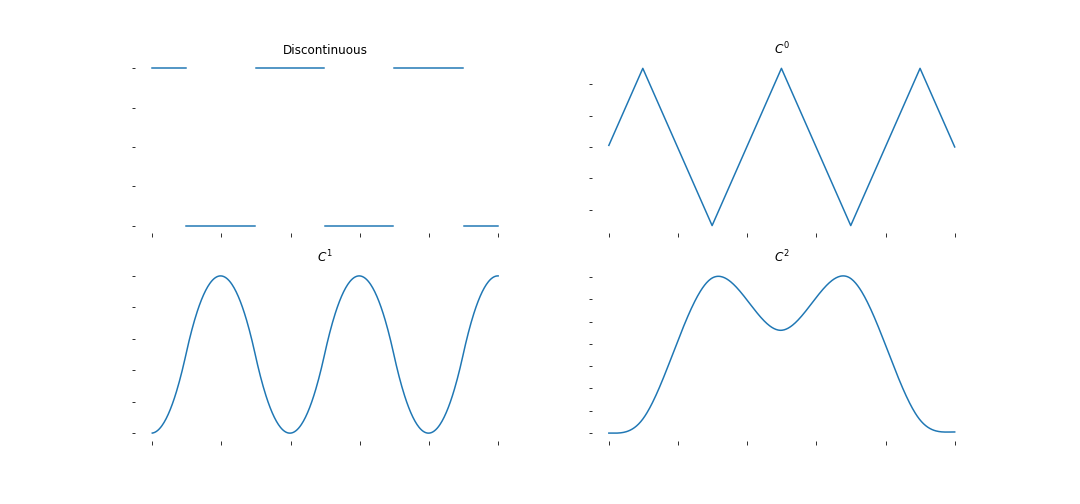
\includegraphics[scale=0.298]{src/4.24 Cn functions.png}
    \caption{$C^n$ functions.}
\end{figure}

There is a difference between having continuous derivatives and knowing what those derivatives are. First order optimisation uses the first derivatives of the objective function with respect to the parameters. These techniques can only be applied if the objective function is:
\begin{itemize}
    \item at least $C^1$ continuous (no step changes anywhere in the function or its derivative), and
    \item differentiable (gradient is defined everywhere).
\end{itemize}
In practice, these constraints are relaxed a bit, as we will see.

Many objective functions satisfy these conditions, and first-order methods can be vastly more efficient than zeroth-order methods. For particular class of functions (e.g. convex), there are known bounds on number of steps required to converge for specific first-order optimisers.

For first-order optimisation, we put a stronger requirement on functions than just $C^1$ continuity and require the functions to be Lipschitz continuous. For a function $\mathbb{R}^n \to \mathbb{R}$ (like the objective function) is equivalent to saying that the gradient is bounded and the function cannot change more quickly than a constant. In particular, there is a maximum steepness.

The Lipschitz constant $K$ for a function $f$ is given by
\[K = \sup \left[\frac{|f(x) - f(y)|}{|x-y|}\right].\]
This is the smallest value larger than every value of the function. A small $K$ means that the function is smooth. If $K = 0$, then it is flat. We do not need to know the value of $K$ to compute the derivative- we just need to know that it exists.

\subsection{Analytical derivatives}
There are manual techniques to compute the derivative and optimise a function $f: \mathbb{R} \to \mathbb{R}$.
\begin{itemize}
    \item Compute the derivative $f'(x)$;
    \item Solve for $f'(x) = 0$- these are turning points/optima of the function;
    \item Check if any of these $x$-values satisfy $f''(x) > 0$. Then, the $x$ value is a local mimum.
\end{itemize}
The following graph illustrates this process.
\begin{figure}[H]
    \centering
    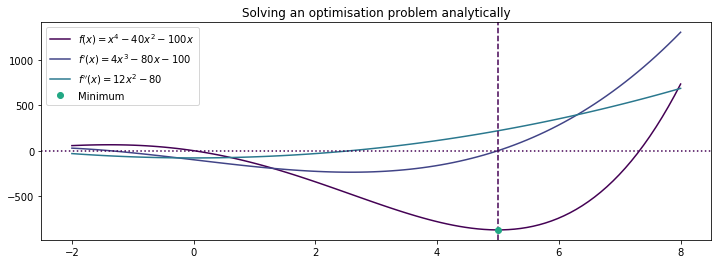
\includegraphics[scale=0.42]{src/4.25 solving an optimisation problem analytically.png}
    \caption{Solving an optimisation problem analytically.}
\end{figure}

In this case, the optimisation process just takes one step- there is no iteration. However, we normally do not have a closed form for the derivative; we can only evaluate the derivative at some point. In this case, we can still dramatically accelerate optimisation by taking steps such that we ``run downhill'' as fast as possible. To do this, we need to be able to compute the gradient at any point on the objective function.

Essentially, for an objective function $f: \mathbb{R}^n \to \mathbb{R}$, we will have a gradient function $f: \mathbb{R}^n \to \mathbb{R}^n$. The gradient function takes in the same parameter. At a given point, the gradient of a function points in the direction where the function increases the fastest. The magnitude of this vector is the rate at which the function is changing.

\section{Gradient Descent}
The basic first-order algorithm is called gradient descent, and involves iterations like in random searching- we start with some initial guess $\theta_0$, and try to converge to the minimum using the equation
\[\theta_{n+1} = \theta_n - \delta \nabla L(\theta_n).\]
Here, $\delta$ is the step size (a hyperparameter)- this might be fixed or adaptive. By construction, the optimiser moves towards the point where the objective function drops most quickly. It is possible that going downhill may not be the fastest route. Nonetheless, gradient descent can be very fast. In gradient descent, we first choose a guess. Then, we loop, using the equation above to minimise the loss function. 

The step size is crucial for convergence. If the step size is too small, then the convergence is too slow, like shown below.
\begin{figure}[H]
    \centering
    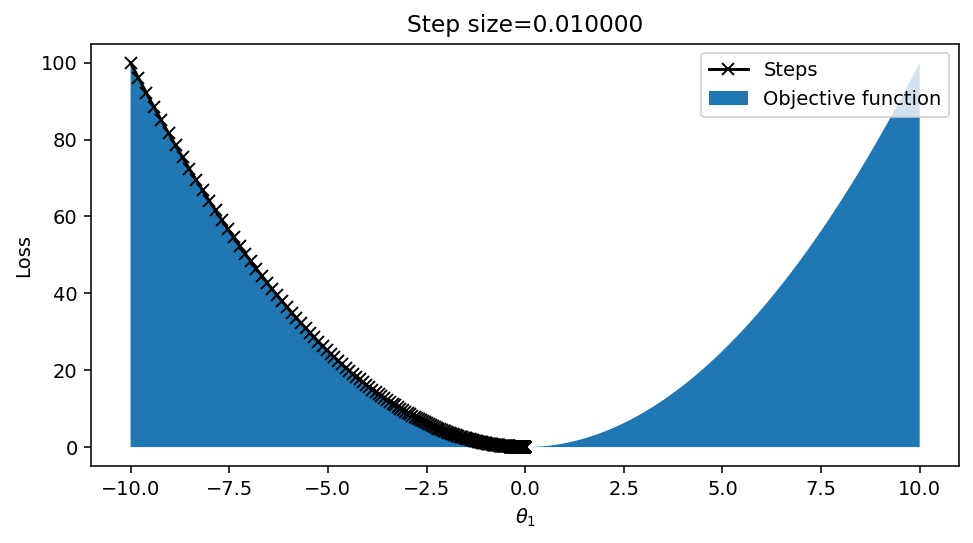
\includegraphics[scale=0.4]{src/4.26 stepsize 0.01.png}
    \caption{Slow convergence by small step size.}
\end{figure}
\noindent Instead, if the step size is big, the optimisation process will oscillate and be slow as well.
\begin{figure}[H]
    \centering
    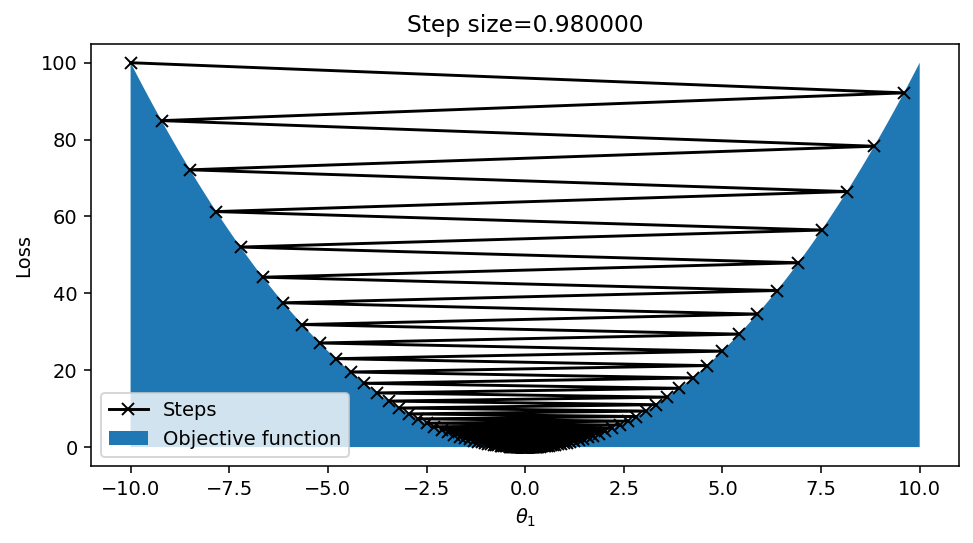
\includegraphics[scale=0.4]{src/4.27 stepsize 0.98.png}
    \caption{Slow convergence by large step size.}
\end{figure}
\noindent Moreover, if the step size is too large, the optimisation process might not have the expected behaviour- it might go past the area where the minima is. The optimality of the step size is related to Lipschitz constant. We typically do not know the constant, so the step size is often set by approximate methods such as line search. We can generalise gradient descent to higher dimensions using the same strategy.

\subsection{Using numerical differences}
To use first-order optimisation, we need to know the derivative of a function. Although there is no direct way of applying this in the real world, we can apply it to the computational model so that it can be optimised. The definition of the derivative at a point is
\[f'(x) = \lim_{h \to 0} \frac{f(x+h) - f(x-h)}{2h}.\]
Using small values for $h$, we could potentially derivative every function. This approach is called numerical differentiation, and these are finite differences.

Numerical difference works fine in 1D cases, as shown below.
\begin{figure}[H]
    \centering
    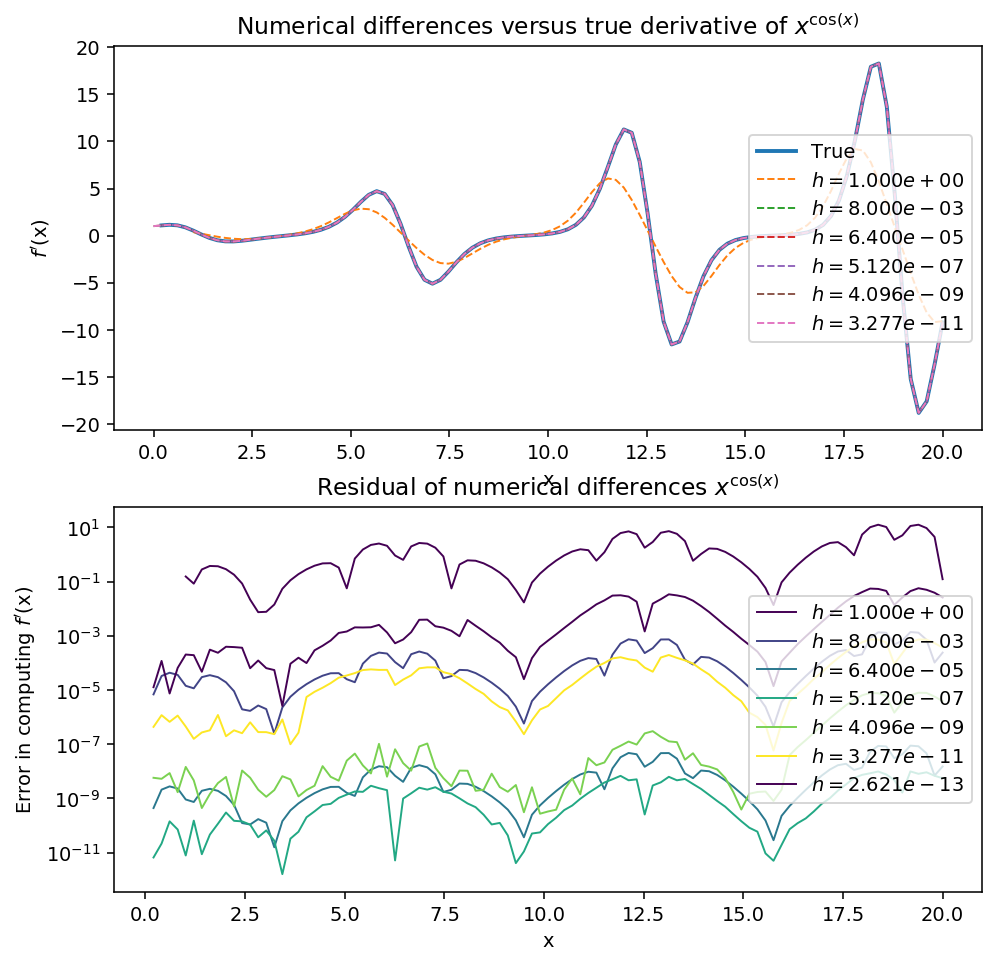
\includegraphics[scale=0.5]{src/4.28 Error in computing f(x).png}
    \caption{Computing the derivative using numerical differences.}
\end{figure}
\noindent In the first graph, we use different values of $h$ to approximate the derivative. The values are quite close most of the time. The second graph shows the difference between the actual derivative and the approximations. 

In the second graph above, we find that as $h$ gets smaller, it is not always the case that the error decreases. This is because there are numerical issues when computing the value
\[\frac{f(x+h) - f(x-h)}{2h}.\]
In particular,
\begin{itemize}
    \item To a big number $x$, we are adding a very small number $h$ (magnitude error).
    \item We are subtracting two numbers $f(x+h)$ and $f(x-h)$ which are about the same (cancellation error).
    \item We divide by $2h$, which is a really small number (division magnification).
\end{itemize}

Moreover, in higher dimensions, the curse of dimensionality reappears. To evaluate the gradient at $\mathbf{x}$, we need to compute numerical differences in each dimension. So, if $\theta$ has one million dimensions, then each individual derivative evlaution would require two million evaluations of $L(\theta)$- this would be too slow and the efficiency of gradient descent would be lost.

Although gradient descent is much more efficient than zeroth-order methods, it has some disadvantages:
\begin{itemize}
    \item The gradient of the objective function must be computable at all points. Automatic differentiation helps with this.
    \item Gradient descent can get stuck at local minima. Gradient descent is meant to just find local minima (only in convex function can we guarantee that a local minimum is global). Random restart and momentum can be used to counter this.
    \item Gradient descent only works with smooth, differentiable objective functions. Stochastic gradient descent allows us to differentiate steep functions by adding noise.
    \item Gradient descent can be slow if the objective function takes a long time to be evaluated. Stochastic gradient descent can massively improve this, given that the objective function can be written as the sum of smaller subproblems.
\end{itemize}

\subsection{Automatic differentiation}
If we had a closed form for the derivative of the objective function, this would be a simple task. However, it is not feasible to work out the closed form when we are dealing with hundreds of dimensions. Automatic differentiation algorithms take a function and automatically construct a function that evaluates the exact derivative of the function at a given point. The package \texttt{autograd} allows us to differentiate a function.

The following figure illustrates the gradient descent to find the line fit through the data above.
\begin{figure}[H]
    \centering
    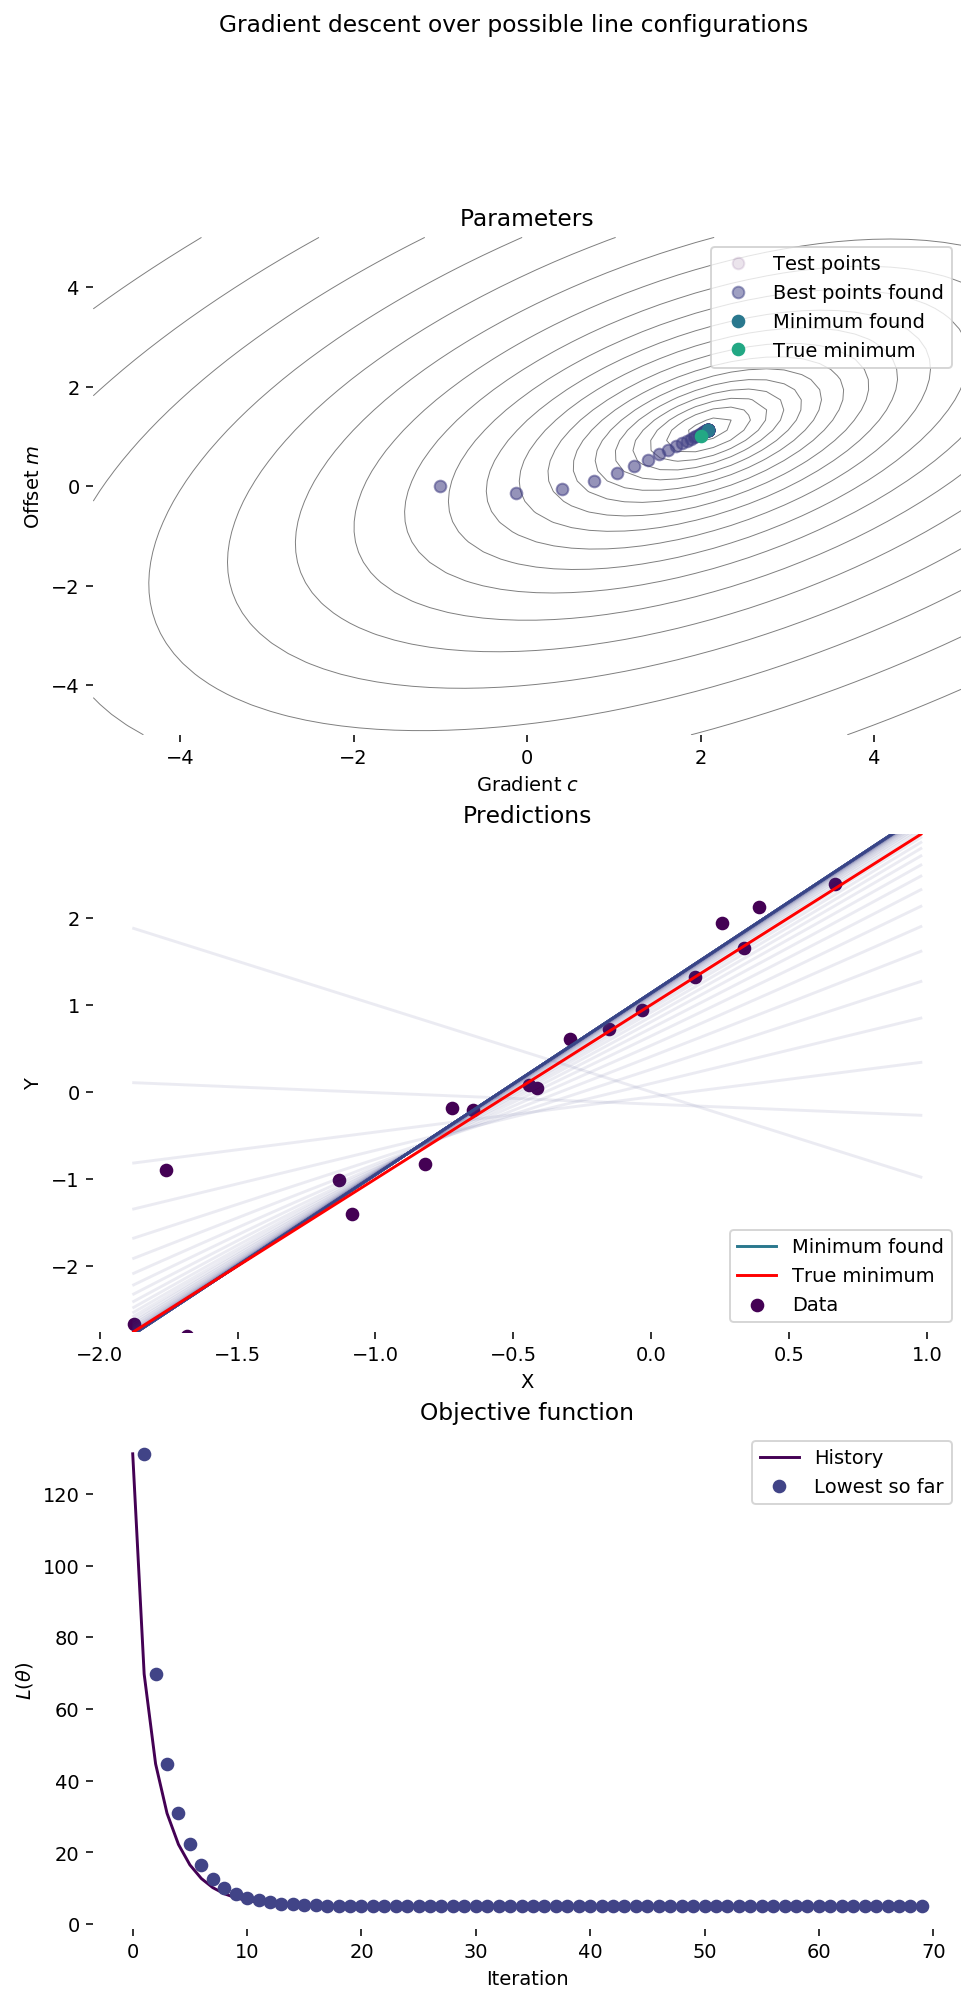
\includegraphics[scale=0.5]{src/4.29 gradient descent line configurations.png}
    \caption{Gradient descent line configurations.}
\end{figure}

\subsection{Limits to automatic differentiation}
We need the function to be differentiable to apply gradient descent. While it is possible to compute first-order derivatives in reasonable time, we will see later it is not feasible in a multi-dimensional setting.

Stochastic relaxation can make an impossibly steep gradient Lipschitz continuous by integrating over many different random conditions. The figure below explains how we relax a non-differentiable function and derive it.
\begin{figure}[H]
    \centering
    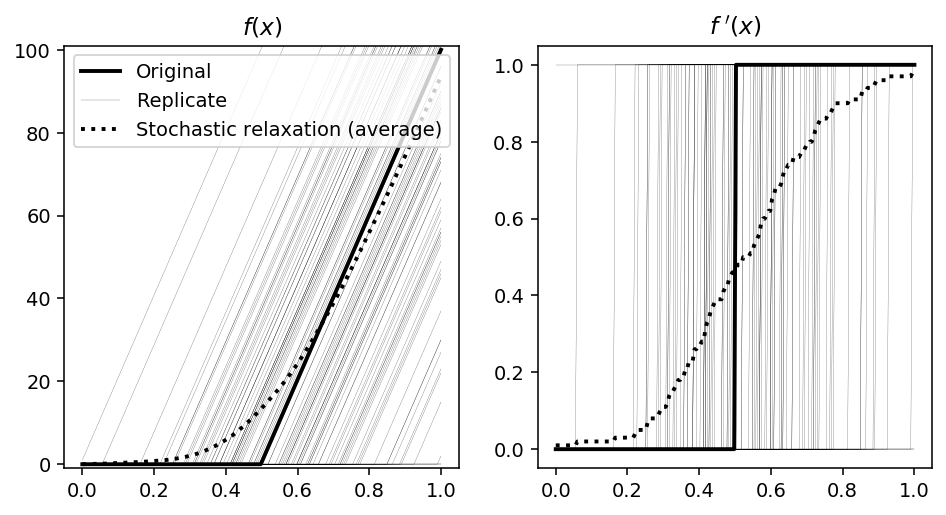
\includegraphics[scale=0.65]{src/4.30 stochastic relaxation.png}
    \caption{Stochastic relaxation of a function.}
\end{figure}

\section{Stochastic Gradient Descent}
In gradient descent, we have to evaluate the function and the gradient during each iteration. This can make the process quite long, e.g. if the data has thousands of dimensions. If we can break the objective function into smaller chunks, then the optimiser can do gradient descent on each of those chunks separately. This might be much faster. This is called stochastic gradient descent, because the step it takes depends on a random part of the objective function.

So, assume that the objective function is of the form
\[L(\theta) = \sum_i L_i(\theta).\]
This is quite common when matching parameters to observations. For instance, in machine learning, we have some training sets $\mathbf{x}_i$ with known outputs $y_i$, and we want to find the parameter vector $\theta$ such that
\[L(\theta) = \sum_i \lVert f(\mathbf{x}_i, \theta) - y_i \rVert\]
is minimised- we try to mimise the distance between the inputs and the outputs elementwise.

Differentiating is a linear operation, meaning that
\[\frac{d}{dx}(a f(x) + bg(x)) = af'(x) + bg'(x).\]
Therefore,
\[\nabla \sum_i \lVert f(\mathbf{x}_i, \theta) - y_i \rVert = \sum_i \nabla \lVert f(\mathbf{x}_i, \theta) - y_i \rVert.\]
So, we can take a subset of the dataset, compute the gradient for each sample/subset. Over time, the randomness will average out. Each subset is a minibatch, and one run (i.e. every dataset has been seen by the optimiser) through the dataset is an epoch.

\subsection{Memory advantages}
Stochastic gradient descent (SGD) has major advantages in terms of memory since computations are only applied to a small number of samples in minibatches. We just compute the gradient on a subsample, and move in that direction. It won't be exactly the right derivative of the whole objective function, but it will be a good approximation.

Particularly on memory-constrained devices such as GPUs, it can be impossible to store the entire dataset on the device. Splitting up into batches can get around this limitation. It can also have advantages with respect to the memory hierarchy- small batches of data may induce fewer cache misses and thus result in enhanced performance.

\subsection{Heuristic enhancement}
SGD can improve the performance of optimisation in terms of objective function decrease. In particular, it reduces the likelihood of getting stuck in minima. This is because random partitioning adds noise to the dataset. This allows the gradient descent to not always go downhill, but also to jump over a hill.

Adding noise is a heuristic approach. It is very effective. This is a limited version of stochastic relaxation- the function gets smoothened out by averaging over random subsamples. This means that if the function is not Lipschitz continuous (or has a high Lipschitz constant), then SGD can still work well when gradient descent wouldn't.

\subsection{Using SGD}
There is no guarantee that SGD will move in the right direction. However, it is normally effective in practice. We can break the linear regression example into multiple subproblems by choosing a few random points at time. The following figure illustrates the SGD to find the line fit through the data.
\begin{figure}[H]
    \centering
    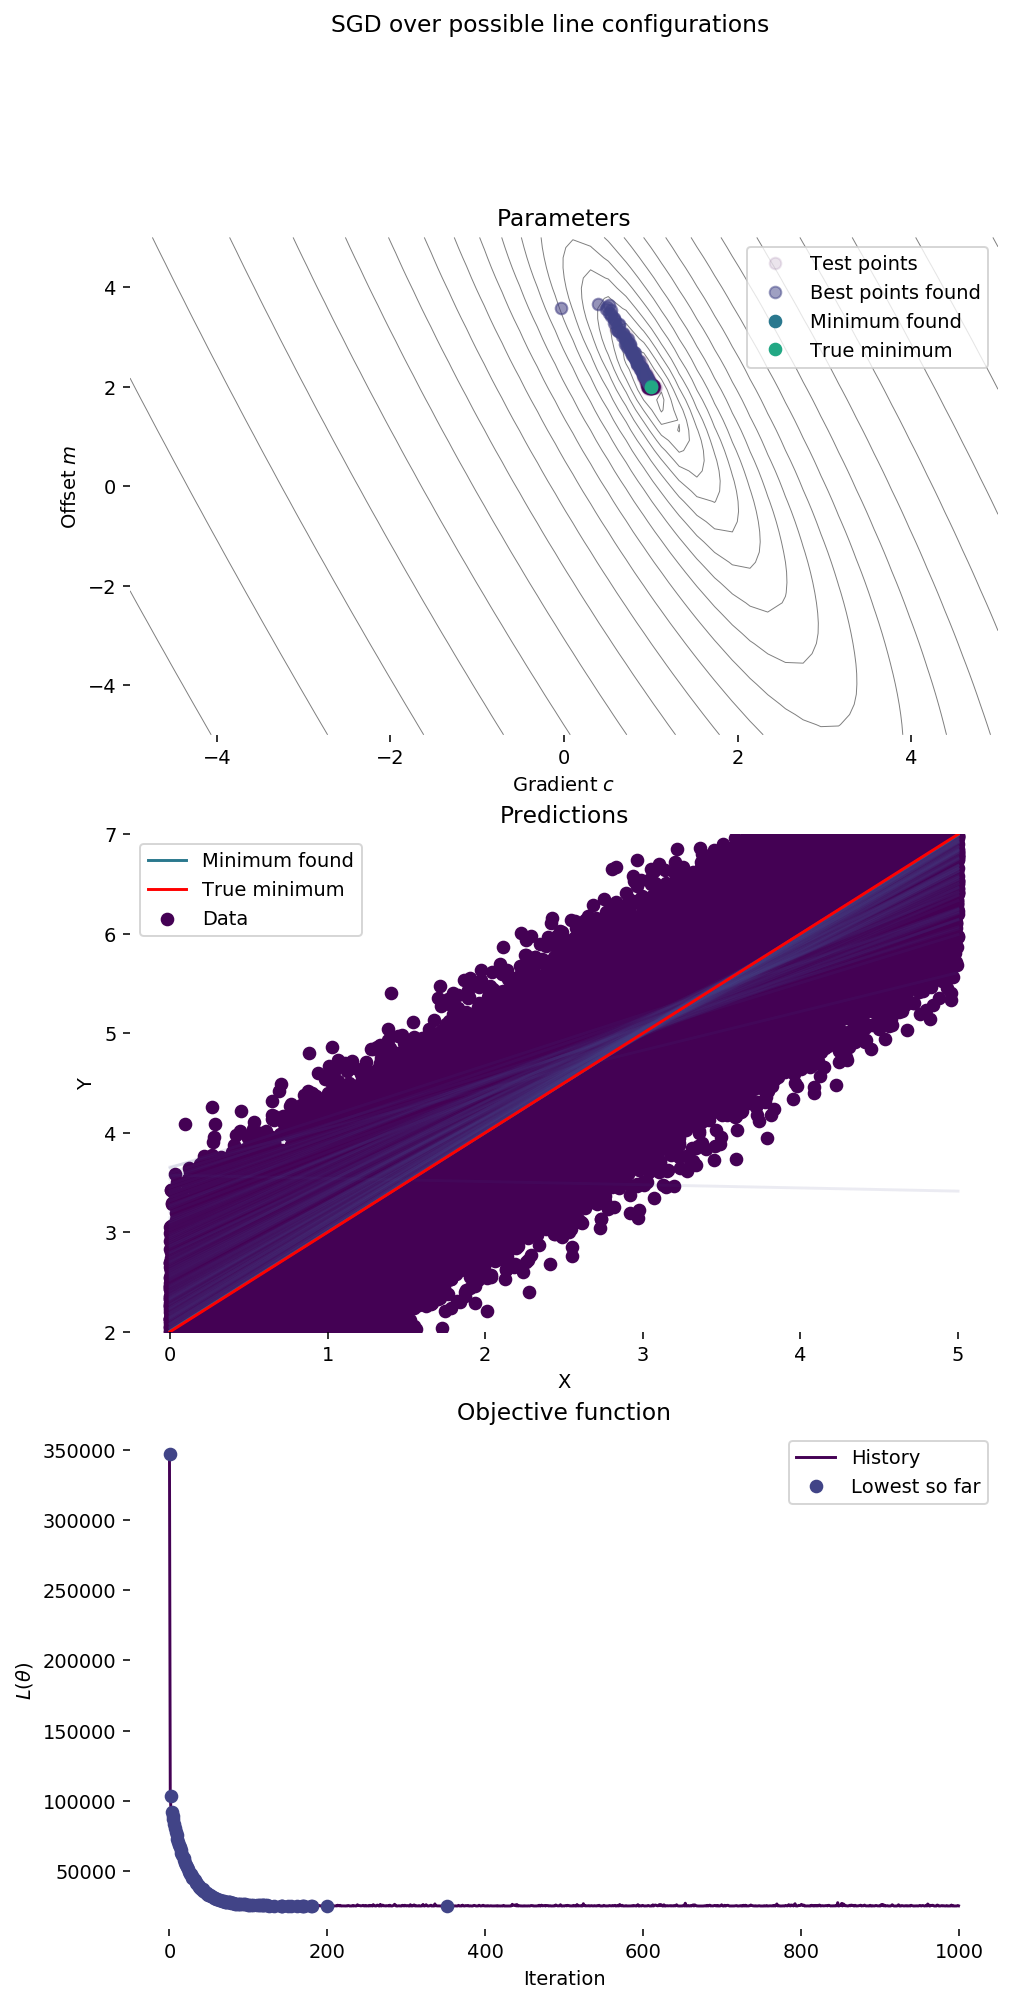
\includegraphics[scale=0.5]{src/4.31 stochastic gradient descent line configurations.png}
    \caption{SGD line configurations.}
\end{figure}

\section{Random Restart and Momentum}
We will try to apply gradient descent to a function which has:
\begin{itemize}
    \item narrow valleys everywhere,
    \item multiple local minima,
    \item a huge ridge through the middle.
\end{itemize}
The graph of such a function is given below.
\begin{figure}[H]
    \centering
    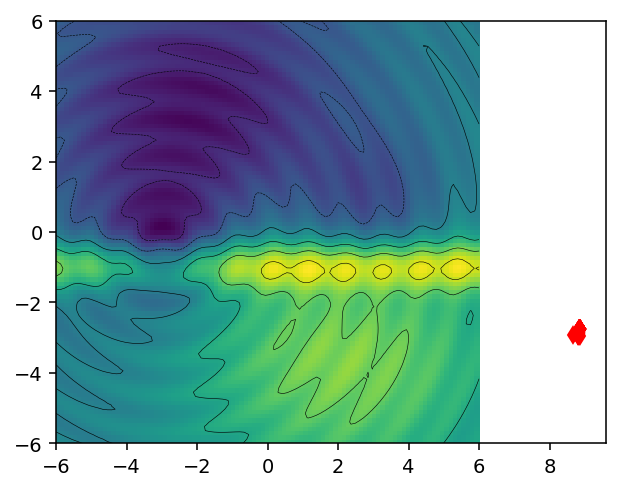
\includegraphics[scale=0.8]{src/4.32 gradient descent horrible function.png}
    \caption{Gradient Descent traceback}
\end{figure}
\noindent Clearly, gradient descent wasn't able to find a minimum. It gets stuck in a valley and wanders in a huge arc, never approaching even the local minima. We can't apply stochastic gradient descent either- the function cannot be broken into multiple segments.

We can use random restart instead. Gradient descent gets stuck at local minima. SGD can help if the minimum isn't too deep. A simple heuristic is to run gradient descent until it gets stuck, and then starting with a different initial condition. We try this many times and try to find the global minimum. We can use random restart with any iterative optimisation algorithm.

Another approach is to use momentum. In real life, if we throw a ball down some hill, it will keep going down even if there are some bumps on the way- it has momentum and will keep going in that direction. We use a similar approach in optimisation algorithms.

This is a form of memory- we introduce velocity $v$. The optimiser moves in this direction. We gradually move the velocity to align with the derivative.
\[v = \alpha v + \delta \nabla L(\theta).\]
In this case, the next value for $\theta$ is:
\[\theta_{i+1} = \theta_i - v.\]
The value $\alpha$ controls the change in velocity. If $\alpha$ is close to 1, there is more momentum in the system. If $\alpha$ is close to 0, this is pretty much the normal gradient descent.

Momentum will give the following traceback with the minimum above.
\begin{figure}[H]
    \centering
    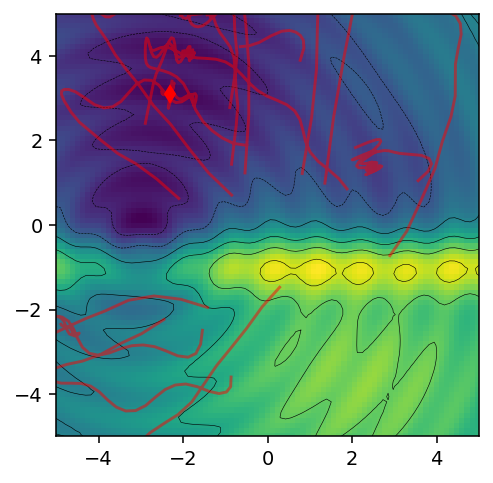
\includegraphics[scale=0.8]{src/4.33 random restart horrible function.png}
    \caption{Mometum traceback.}
\end{figure}

\section{Second order derivatives}
The first order derivatives represents the slope of the function. The second order derivatives represent the curvature of the function. For every parameter component $\theta_i$, the Hessian stores how the steepness of every other $\theta_j$ changes.

If a person is on a hill,
\begin{itemize}
    \item The altitude is the value of the objective function.
    \item The parameters that can change are position (e.g. north, south, east, west).
    \item The gradient vector is the change in altitude as the person steps in one of the two directions. This is the local steepness.
    \item The Hessian captures how much steeper the hill gets stepping in some direction. There are 2 independent directions, so the Hessian is a $2 \times 2$ matrix.
\end{itemize}

The gradient vector captures the first order derivatives, while the Hessian matrix captures the second order derivatives. For every pair of dimensions, there is an entry in the Hessian matrix. The Hessian matrix captures how gradients of a function vary with respect to each other.

For a 2D surface, the gradient vector specifies the normal of the plane tangent to the surface at a given point. The Hessian matrix specifies a quadratic function (a smooth curve with one minima) following the curvature of the surface.

\subsection{Eigenvalues of the Hessian}
The eigenvalues of the Hessian allow us to characterise the type of stationary point. In particular,
\begin{itemize}
    \item if all the eigenvalues are strictly positive (i.e. positive definite), then the point is a minimum;
    \item if all the eigenvalues are strictly negative (i.e. negative definite), then the point is a maximum;
    \item if eigenvalues have mixed signs, the point is a saddle point;
    \item if the eigenvalues are all positive/negative, but with some zeroes, the matrix is semidefinite and the point is a plateau/ridge.
\end{itemize}

\subsection{Second order optimisation}
Second order optimisation uses the Hessian matrix to jump to the bottom of each local quadratic approximation in a single step. This can skip over flat plains and escape from saddle points that slow down the gradient descent. Second-order derivatives are much faster in general than first-order methods. The following graph compares some optimisation algorithms.
\begin{figure}[H]
    \centering
    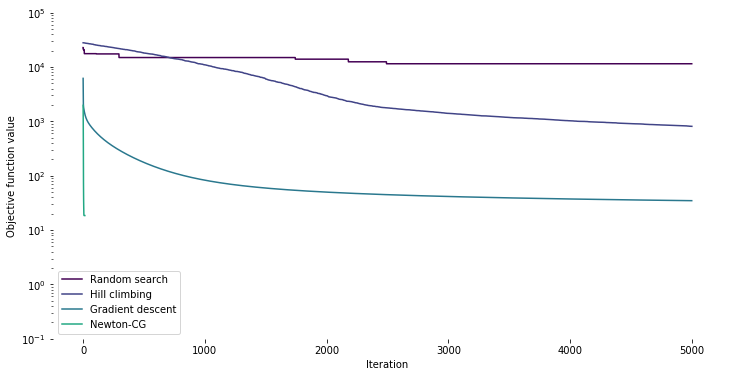
\includegraphics[scale=0.45]{src/4.34 comparing optimisation algorithms.png}
    \caption{Comparing optimisation algorithms.}
\end{figure}
\noindent Random searching does quite a bad job. Hill climbing does decrease the objective function significantly, but is still not that good. Gradient descent does quite a good job, but Newton-CG (a second order optimisation algorithm) does a much better job.

Second-order optimisation doesn't work in higher dimensions. Evaluating the Hessian takes $d^2$ computations, and $d^2$ storage. This isn't possible if $d$ is huge.

So, second order optimisation can move much more quickly through saddle points and plateaus than first order methods like gradient descent. However, it is not possible to use second order optimisation in high dimensions due to the curse of dimensionality.


\end{document}